% arara: pdflatex
% arara: bibtex
% arara: pdflatex
% arara: pdflatex

\documentclass[natbib,a4paper,preprint,number,sort&compress,times]{elsarticle} 

\usepackage{preamble}

\makeatletter
\def\Cline#1#2{\@Cline#1#2\@nil}
\def\@Cline#1-#2#3\@nil{%
  \omit
  \@multicnt#1%
  \advance\@multispan\m@ne
  \ifnum\@multicnt=\@ne\@firstofone{&\omit}\fi
  \@multicnt#2%
  \advance\@multicnt-#1%
  \advance\@multispan\@ne
  \leaders\hrule\@height#3\hfill
  \cr}
\makeatother

\iffalse
1) (Anna) Ground framework terms in table 1 deeper in section 2 / relate them more closely to the related work. Use words from last line of table 1 in section 2.
2) (Christian) Stress that we focus on serendipity in the system, not system supporting serendipity in person. Stress that we do not programme serendipity, but serendipity potential. Refactor text on serendipity as a service. Cf. creativity support tools and computational creativity. We adopt similar analogy.
3) (Joe) In section 3, define different components based on (i) theoretical (deepen) and (ii) CS literature (formal). The definition of components and how they're technically realised currently. (One stage, drawing implementations from many systems). DONE
4) (ALL) Describe applications of this in section 4, not evaluating potential anymore. How could serendipity in system benefit researchers / users? (One system - compared against all stages from framework) Potential projects to discuss: painting fool (involve Simon!), coinvent, Mexica, etc.
5) (Christian) Clarify major contributions in introduction / conclusion, rewrite abstract to guide our work (NB subsection added by AJ in Section 5 for conclusions to go in)
6) (Christian) Draft figure to summarise findings in sec. 3.
7) (Anna) revise section 5 to not be a wall of text - (make space for Christian to clarify major contributions as a conclusion - DONE)
\fi

%%% Hack to get showframe to work with landscape pages, from stack exchange
%%% https://tex.stackexchange.com/questions/115908/geometry-showframe-landscape -JC
%% Remove this...
\usepackage{geometry}
%% and replace with the following...

%% \usepackage[
%%  outer=25mm,
%%  inner=35mm,
%%  vmargin=20mm,
%%  includehead,
%%  includefoot,
%%  headheight=15pt,
%%   showframe
%% ]{geometry}

%% \usepackage{pdflscape}

%% \makeatletter
%% \newcommand*{\gmshow@textheight}{\textheight}
%% \newdimen\gmshow@@textheight
%% \g@addto@macro\landscape{%
%%   \gmshow@@textheight=\hsize
%%   \renewcommand*{\gmshow@textheight}{\gmshow@@textheight}%
%% }
%% \def\Gm@vrule{%
%%   \vrule width 0.2pt height\gmshow@textheight depth\z@
%% }%
%% \makeatother

%%% end of showframe hack

\begin{document}

\begin{frontmatter}

\iffalse
I write concerning your submission to the Artificial Intelligence journal titled “Modeling Serendipity in a Computational Context”.  After careful consideration, we have decided to decline your article for publication in the Artificial Intelligence Journal.  

The topic of the paper is of great interest, as a broad understanding of intelligence must address such concepts as serendipity, creativity, innovation, and discovery.  As the authors point out, there are specific references to such notions in the AI literature but an overarching framework has been lacking. This is the focus of the article, which culminates in a framework with six phases where selected works from the literature are situated and discussed.

The framework itself is valuable in that it lays the foundations for an understanding of the different aspects involved in serendipity and creativity.  However, the proposed framework lacks a formal computational basis that would be needed in order to make a strong contribution of impact to the field.  

A formalism would be a key mechanism to connect with artificial intelligence research.  For example, while the Perception, Attention, Focus, and Explanation phases were not surprising, it is hard to  see that the proposed "bridge" phase to bring the serendipitous realization into a new problem area would be required.  In addition, it is not clear that one would see that phase in all problems where I would consider serendipity to occur.  For example, I would consider representation changes to be often designed through serendipity and not requiring a bridge phase to link to a new domain.  Conversely, I would consider other serendipitous discoveries having their start in that bridge phase, for example beginning the process by searching for analogies and then proceed with the Focus and Explanation phases.  Although the paper states that one can go back to previous phases, it does not mention whether and how one could start in any of them.  A clear formalism would clarify the issues raised here and be better positioned to influence the field.

A formalism would also help define what is meant by different terms and clarify the concepts.  The main concepts identified as key to describe the different phases and their components are quite abstract, and their definitions are provided using terms that are also abstract.  For example, it is not clear how "context", "explanation", and "contextual explanation" relate or if they overlap.  Or the elaboration of an "inspiration" stage into "incubation" and "insight".

Further formalization would also push the computational basis for the work and increase its impact.  For example, analogies are rightly recognized by the authors as a key component of serendipity.  It is discussed as a heuristic in the Bridge phase.  The work that is cited on analogy is not a formalized analogical reasoning.  It would be helpful to understand how this phase would map to computational models of analogy, such as Deidre Gentner's Structure Mapping or Manuela Veloso's derivational and transformational analogy.  Both are well-know, implemented computational frameworks for analogy, and describing how serendipity would map to such formalizations would increase the impact of the ideas presented in the article.

The paper is rightly situated by the authors as philosophical foundations of AI and commonsense reasoning.  Those areas are of interest to the journal, but the papers we accept must have a clear contribution to artificial intelligence.  I have consulted with others about the article, and I am perhaps the most appreciative of all about the ideas it puts forward.  I suspect the most interesting part of the article for artificial intelligence researchers will likely be that it draws from implemented approaches and architectures to provide examples of where serendipity and creativity can be glimpsed. Examples are drawn from some of the literature in learning, robotics, and cognitive architectures.  While this would be of interest to journal readers, it is not enough of a contribution in itself to grant acceptance.

Thank you for submitting your work to the Artificial Intelligence journal.  We get a large number of submissions, and our goal is to identify those submissions that will have an impact in the field.  I hope that you will continue to keep the journal in mind as a potential outlet for your best work.

\hfill  Patrick Doherty

\clearpage
\fi

% TITLE INFORMATION
\title{Modelling Serendipity in a Computational Context}

%% \thanks{This research was supported by the Engineering and Physical Sciences Research Council through grants EP/L00206X, EP/J004049 as well as EP/L015846/1 and the Future and Emerging Technologies (FET) programme within the Seventh Framework Programme for Research of the European Commission, under FET-Open Grant numbers: 611553 (COINVENT) and 611560 (WHIM).}

\author[A,G]{Joseph Corneli\corref{cor1}\fnref{fn1}}
\ead{joseph.corneli@ed.ac.uk}
\author[B]{Anna Jordanous}
\ead{a.k.jordanous@kent.ac.uk}
\author[C]{Christian Guckelsberger}
\ead{christian.guckelsberger@qmul.ac.uk}
\author[D]{Alison Pease}
\ead{a.pease@dundee.ac.uk}
\author[C,E]{Simon Colton}
\ead{s.colton@qmul.ac.uk}

\cortext[cor1]{Corresponding author}
\fntext[fn1]{Present address: School of Informatics, University of Edinburgh, 10 Crichton St, Edinburgh EH8 9AB, UK}

\address[A]{School of Informatics, University of Edinburgh, 10 Crichton St, Edinburgh EH8 9AB, UK}
\address[B]{School of Computing, University of Kent, Chatham Maritime, Medway, Kent ME4 4AG, UK}
\address[C]{School of Electronic Engineering and Computer Science, Queen Mary University of London, Mile End Road, London E1 4NS, UK}
\address[D]{School of Science \& Engineering, University of Dundee, Dundee DD1 4HN, UK}
\address[E]{Sensilab, Monash University, 900 Dandenong Road 
Caulfield East Victoria 3145, 
Australia}
%% \institute{
%% J.~Corneli\\
%% School of Informatics, University of Edinburgh\\
%% Email: joseph.corneli@ed.ac.uk \\[2mm]
%% C.~Guckelsberger \and S.~Colton\\
%% Department of Computing, Goldsmiths, University of London\\
%% Email: c.guckelsberger@gold.ac.uk, s.colton@gold.ac.uk\\[2mm]
%% A.~Jordanous\\
%% School of Computing, University of Kent\\
%% Email: a.k.jordanous@kent.ac.uk\\[2mm]
%% A.~Pease\\
%% School of Science and Engineering, University of Dundee\\
%% Email: a.pease@dundee.ac.uk\\}
% \date{\vspace{-1in}}%\today - revised version due 8 weeks from 20/04/2016, so before 15/06/2016
%\address[G]{Department of Computing, Goldsmiths, University of London, New Cross, London SE14 6NW, UK}

\begin{abstract}
%% Overall definition
We understand the term serendipity to describe a creative process that
develops, in context, with the active participation of a creative
agent, but not entirely within that agent's control.
%% Section 1
While a system cannot be made to perform serendipitously on demand,
nevertheless, we argue that its \emph{serendipity potential} can be
increased by means of a suitable system architecture and other design choices.
%% Section 2 
We distil a unified description of serendipitous occurrences from
historical theorisations of serendipity and creativity.  Whereas most
existing research that considers serendipity in a computing context
deals with serendipity as a service, we relate theories of serendipity
to artificial intelligence practice and the development of autonomous
systems.

\end{abstract}

\begin{keyword}
Serendipity \sep Discovery Systems \sep Automated Programming \sep Recommender Systems \sep Computational Creativity \sep Autonomous Systems \sep Predictive Processing
\end{keyword}

\end{frontmatter}

% \titlerunning{Modelling serendipity in a computational context}
%\authorrunning{~}

%\maketitle

\thispagestyle{plain}
\pagestyle{plain}

\clearpage


% * <annajordanous@gmail.com> 2017-12-15T18:35:21.454Z:
%
% ^.
%\tableofcontents

%\newpage

%\begin{abstract}
%% INNOVATIVE
%% Serendipity has played a key role in fundamental scientific and
%% technical advances, but its potential to contribute to discovery and
%% innovation by computational systems is often downplayed.
%% %% CONTRIBUTION TO UNDERSTANDING AND KNOWLEDGE
%% The concept of serendipity has, however, been taken up by researchers
%% in information science, for whom it denotes the development of systems
%% that support happy chance discoveries for their users.
%% %% NEW ARGUMENTS
%% rticle, we advance a novel perspective, shifting the focus
%% from ``serendipity as a service'' to artificial systems that
%% themselves catalyse, evaluate and leverage serendipitous occurences.
%% INTERPRETATIONS OR INSIGHTS
While a system cannot be made to perform serendipitously on demand,
nevertheless, we argue that its ``serendipity potential'' can be
increased by means of a suitable system architecture.
%%%
%%%
%% %% IMAGINATIVE SCOPE
%% Rather than relying on the system's user to contribute mental or
%% physical effort, such systems are required to be suitably self-reliant
%% in relevant cognitive, conative, and affective respects.
%% %% ASSEMBLING OF INFORMATION IN AN INNOVATIVE WAY
%% Based on a survey of theoretical literature, we advance a %sequential
%%  model of serendipitous occurrences in a computational context that
%% stresses the role of creativity, invention and discovery.
%% %%
%% We also survey existing implementations and describe how the ideas
%% they embody could be reused to realise our framework's individual
%% components.
%% %%
%% This allows us to assess the current progress towards systems that
%% exhibit serendipitous behaviour, and the gaps that lie between current
%% systems and a full implementation of the model.
%%
%% NEW THEORETICAL FRAMEWORKS AND CONCEPTUAL MODELS
We elaborate a cognitively-inspired model of serendipity potential,
described in six phases:
%%
\emph{perception}, \emph{attention}, \emph{interest},
\emph{explanation}, \emph{bridge}, and \emph{valuation}.
%%
Earlier phases can be returned to from later phases as a creative
process develops, in context, with the active participation of a
creative agent, but not entirely within that agent's control.
%%
We evaluate the model by applying it to existing systems, and point to
further applications in automated programming, recommender systems,
and computational creativity.
%%
We conclude that equipping computational systems with the potential for serendipity is widely applicable across
different artificial intelligence applications.
%% %% ENHANCEMENT OF KNOWLEDGE, THINKING, UNDERSTANDING
%% We discuss how designers and could benefit from a full implementation
%% of ``serendipity in the system'', and some of the challenges that
%% designing for serendipity raises.
%% %% PRACTICE
%% Since such systems are not strictly controlled by the programmer,
%% their long-term behaviour raises a number of practical and ethical
%% concerns.  In particular, one key aspect of the framework is that it
%% envisions systems that invent their own evaluation functions.
%% %% COHERENCE
%% We argue that the concept of serendipity can be used as a safeguard in
%% meta-evaluations that ensure the system's long-term behaviour
%% benefits its user and other stakeholders over the long run.
%%% I've run out of steam here, but we should deal with the
%%% following issues in the discussion and conclusion, and then
%%% come back to the abstract and add further details. -JC
%% ANALYTICAL POWER
%% DEPTH OF SCHOLARSHIP
%% APPROPRIATE ENGAGEMENT WITH OTHER RELEVANT WORK
%% PROFOUND INFLUENCE
%% INSTRUMENTAL IN DEVELOPING NEW THINKING
%% PRACTICES
%% PARADIGMS
%% POLICIES
%% A MAJOR EXPANSION OF THE RANGE AND THE DEPTH OF RESEARCH
%% OUTSTANDINGLY NOVEL
% 4-6 keywords
%% \keywords{Serendipity,
%% Discovery Systems,
%% Computational Creativity,
%% Recommender Systems,
%% Automated Programming}
\end{abstract}


\iffalse
%OLD ABSTRACT
Building on a survey of previous theories of serendipity and
creativity, we advance a phased model of serendipitous occurrences. We distinguish between serendipity as a service and serendipity in the system itself, clarify the role of invention and discovery, and provide a measure for the serendipity potential of a system.
%%%
While a system 
can arguably not be guaranteed to be serendipitous, it can have a 
high potential for serendipity. Practitioners can use these theoretical tools to evaluate a
computational system's potential for
unexpected behaviour that may have a beneficial outcome.
%%%
In addition to a qualitative features of serendipity potential, the
model also includes quantitative ratings that can guide development
work. We show how the model is used in three case studies of existing
and hypothetical systems, in the context of evolutionary computing,
automated programming, and (next-generation) recommender systems.
From this analysis, we extract recommendations for practitioners
working with computational serendipity, and outline future directions
for research.
\fi

\newpage


%\bigskip
%\maketitle
%\linenumbers
% * <annajordanous@gmail.com> 2017-12-15T18:35:29.228Z:
%
% ^.
% * <annajordanous@gmail.com> 2017-12-15T18:35:27.117Z:
%
% ^.
\setcounter{footnote}{0}

%% It occurs to me that the six sections of the paper could be used
%% to demonstrate the six sections of the model! -Joe Dec 31 2018

\ifdraft{\tableofcontents
\clearpage
}{}

\section{Introduction} \label{sec:why-this-matters}
Current thinking about AI policy points out considerations related to verification, validity, security and control that can reduce the incidence of surprising behaviour in autonomous systems \cite{research-priorities}, but, so far, less attention has been given to features that would allow these systems to make beneficial use of surprises they encounter in the world. 
%
The scope and meaning of system autonomy has been debated since the dawn of the computing age.  Luigi Menabrea \cite[p.~689]{menabrea1842sketch} wondered whether Babbage's Analytical Engine might be made to interpret its results, if it was endowed with a suitable symbolic framework.
Ada Lovelace famously characterised the stengths and the limitations of the Engine: ``It can do whatever we know how to order it to perform'' \cite[p.~722]{lovelace}.  She also presciently observed that the complexity of program operations would push the limits of human understanding, since it involves ``several distinct \emph{sets of effects} going on simultaneously; all in a manner independent of each other, and yet to a greater or less degree exercising a mutual influence'' (\emph{ibid.}, p.~710; emphasis in original).
%% \begin{quote}
%% ``\emph{There are frequently several distinct \emph{\textbf{sets of effects}} going on simultaneously; all in a manner independent of each other, and yet to a greater or less degree exercising a mutual influence. To adjust each to every other, and indeed even to perceive and trace them out with perfect correctness and success, entails difficulties whose nature partakes to a certain extent of those involved in every question where \emph{\textbf{conditions}} are very numerous and inter-complicated; such as for instance the estimation of the mutual relations amongst \emph{\textbf{statistical}} ph\ae nomena, and of those involved in many other classes of facts.}'' \cite[p.~710]{lovelace}~{[}emphasis in original{]}
%% \end{quote}

A hundred and twenty five years later, Marvin Minsky described the state of affairs in programming practice.  ``When a program grows in power by an evolution of partially-understood patches and fixes, the programmer begins to lose track of internal details and can no longer predict what will happen'' \cite{minsky1967programming}.
% https://web.media.mit.edu/~minsky/papers/Why%20programming%20is--.html
In the early twenty first century, neural programs are now routinely evolved by computational means, resulting in code and behaviour that no one can claim to fully understand.  The systems that Turing called \emph{learning machines} \cite{turing1950mind} are now part of everyday life.  Although these systems have mastered constrained domains such as Chess and Go, more powerful applications, such as language learning and human-level performance in mathematics \cite{turing1948intelligentreport} are not yet fully developed.     
%%
Like Turing, \citet[p.~2015]{sloman2008well} highlights ``interactions with a complex environment'' as a prerequisite for learning mathematics.    

As a route to an improved understanding of autonomous systems, our goal in this paper will be to model \emph{serendipity} in computationally-feasible terms. In response to a classic objection to the generation of ``pure serendipity'' by computational means \cite{van1994anatomy},  we embrace the concept of \emph{serendipity potential}.
%In Section \ref{sec:literature-review}, 
We draw on a review of prior literature on serendipity and related concepts such as discovery, invention, creativity, and insight.  We assemble a unified framework that summarises the logical structure of serendipitous occurrences.
% In Section \ref{sec:our-model},
This leads us to a process-oriented model of systems with serendipity potential with six constituent phases:
\emph{perception}, \emph{attention}, \emph{interest}, \emph{explanation}, \emph{bridge}, and \emph{valuation}.
We draw on concepts from cognitive science and philosophy to define these terms, and examine examples of systems that implement the features of the model.
% In Section \ref{sec:system-analysis},
Our discussion outlines directions for future development.

\section{Background} \label{sec:background}

The concept of serendipity has been adopted for users' benefit by many subfields of computer science, including information retrieval \cite{Toms2000, Andre:2009:XSP:1518701.1519009}, recommender systems \cite{kotkov2016survey} and planning \cite{muscettola1997board, chakraborti2015planning}. For example, the {\sf SerenA} project, developed by \citet{maxwell2012designing}, aimed to support users in forming bridging connections from an unexpected encounter to a previously unanticipated but valuable outcome by drawing on linked data from the web. With {\sf Auralist}, \citet{Zhang2011} present a case-study on serendipity in music recommendation: they increase the unexpectedness of their recommendations by means of a declustering algorithm on item popularity and user profile similarity. \citet{chakraborti2015planning} develop a formal account of planning for serendipity in human-robot interaction: they describe an urban search and rescue scenario where a person must conduct triage in a certain room, and then experiences serendipity when the robot intercepts ``him with a medkit in the hallway so he need not fetch one himself.''

There is a strong bias in the existing technical literature towards ``serendipity as a service'', i.e. to leveraging computer systems to support and catalyse a serendipitous experience in the user. In this article, we propose to switch perspectives from such ``serendipity as a service'' to ``\emph{serendipity in the system},'' where artificial systems catalyse, evaluate and leverage serendipitous occurrences themselves. This perspective shift requires a more nuanced understanding of serendipity.  One strategy would be to consider a reversal of roles in which a person contributes to a system's experience of serendipity in some suitable sense.  However, our central goal is to theorise, and indicate in broad terms how to engineer systems which do not depend on such support by people, but which have the capacity to detect, evaluate and use serendipitous events without user intervention.  Why might such features be useful?  Consider the following point raised by \citet{delamaza1994generate}: ``How disastrous it would be if a discovery system's greatest discovery was `not noticed' because a human did not have the ability to recognise it!''

We fully agree with van Andel that an artificial system cannot be guaranteed to engage in serendipitous findings \cite{van1994anatomy}, just as a person cannot deliberately force serendipity to happen on demand.  However, we still believe that serendipity can happen independently of human intervention within an artificial system, and that the ``\emph{serendipity potential}'' of such a system can be increased by means of a suitable system architecture. 
We will frame our analysis in terms of a current theory in cognitive science known as \emph{predictive processing} (for a recent review, see \cite{newen2018oxford}).  The main hypothesis in this line of work is that perception and action are driven by those data which are found to be unexpected.  Alongside in-built faculties and predispositions, previous experience shapes expectations.  Data that differs from the expected provokes a response: some responses support homeostasis, others drive curiosity, and so on.

Although it is finding new applications in a range of areas, including AI and robotics (see, e.g., \citet{DBLP:journals/corr/McGregorBB15,10.3389/frobt.2018.00021,thornton2017predictive}), the predictive processing framework is also conveniently glossed as ``the latest incarnation of an approach to perception and cognition initiated by Kant and refined by Helmholtz'' \cite{swanson2016predictive}.  Some of this philosophical groundwork is relevant to our current concerns.  Kant had contended that ``reason has insight only into what it itself produces according to its own design''---and he disparaged the notion of learning from accidental observations absent ``a previously thought out plan'' \cite[p.~20]{kant1929critique}.  In light of our current considerations it is also natural to wonder what, if anything, can be learned from a previously thought out plan in the absence of accidents.  Kant allowed for new rules to be invented via \emph{reflective judgement}, in a process somewhat akin to unsupervised learning \cite[p.~265]{kant1987critique}.  Reflection is a ``subjective principle governing the purposive use of our cognitive powers'' \cite[p.~266]{kant1987critique}.  Recent work within the predictive processing paradigm posits the subjective sense of `grip' as a driver for curiosity \cite{Kiverstein2017}.

As we adapt to the world, humans create ``new cognitive niches, new
training regimes and designer environments in which to
think'' \cite[p.~265]{pittphilsci10470}.  Herbert Simon
conceptualised \emph{design} as ``the generation of alternatives and,
then, the testing of these alternatives against a whole array of
requirements and
constraints'' \cite[pp.~128--129]{simon1996sciences}. This combination
of bottom-up production and top-down testing is similar to what goes
on in predictive processing theories.  The model of serendipity that
we will develop in Section \ref{sec:our-model} has structural
similarities to a model of design science research developed
by \citet{Peffers:2007:DSR:1481765.1481768}.  However, whereas their
Design Science Research Methodology begins with a problem, in our
model of serendipity, a problem only emerges after several processing
steps.  Our model may be understood as an alternative account of
design processes that more fully embraces phenomena.
%% As we indicated above, we do not think it is possible to design serendipity, though it has been recognised that it is possible to design \emph{for} serendipity \cite{newman2002designing}.  In light of the fact that, e.g., ``the basal ganglia is connected to the cortext by at least five separate circuits''
%so that ``online cognitive function cannot be assigned to either the cortical or subcortical component, but instead emerges from their tight coordination''

%% \begin{figure}
%% 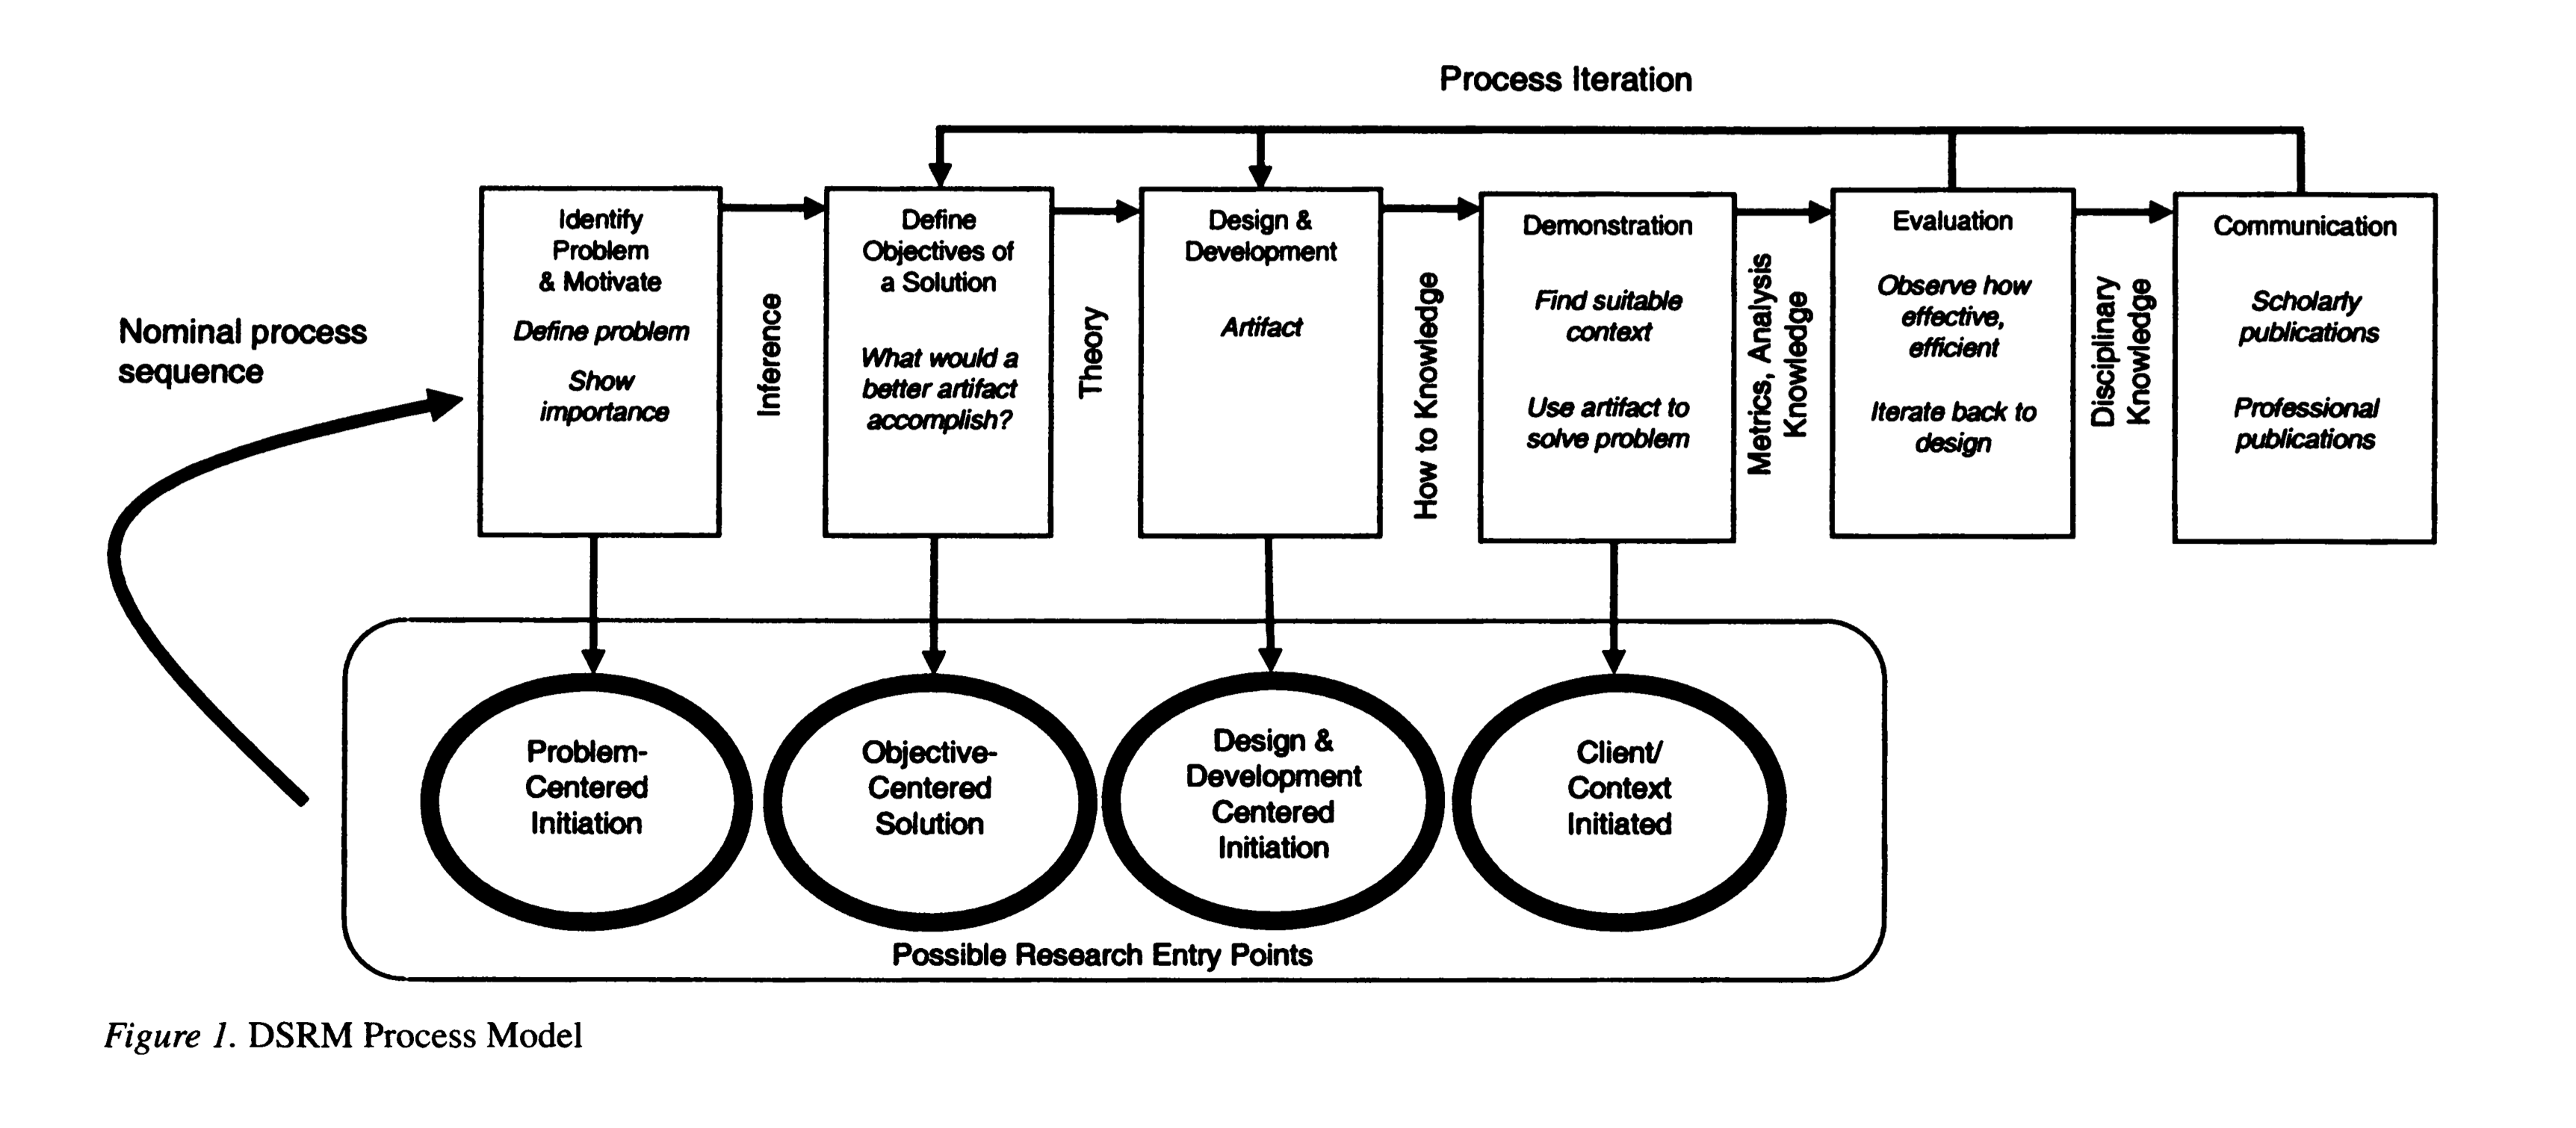
\includegraphics[width=\textwidth,trim={0 3cm 0 0},clip]{pfeffers}
%% \caption{\citet[p.~54]{Peffers:2007:DSR:1481765.1481768} Design Science Research Methodology (DSRM)\label{fig:dsrm}}
%% \end{figure}

\section{The structure of serendipitous occurrences}
\label{sec:literature-review}

To capture the intricate concept of serendipity in a model that is amenable to computational implementation, we first need a thorough understanding of the concept.  Our objective in this section is therefore to identify the factors common to existing theories of serendipity in one unified interpretation.  We will draw on related conceptualisations of \emph{creativity}, a theme that has drawn considerable attention in artificial intelligence research (cf.~\cite{boden1998creativity,colton2009computational,mccormack2012computers}).  


% This motivates our return to the theoretical literature and consider both the origins and development of the serendipity concept as foundation for our framework. We consequently start with a survey of definitions and the etymology of serendipity. We then describe how serendipity is intertwined with creativity, and eventually juxtapose our findings to derive the components of our framework. %Not even unambiguously defined within domain of recommender systems (cf. Lu et al., 2012). Most popular is definition by Herlocker et al.: „A serendipitous recommendation helps the user find a surprisingly interesting item he might not have otherwise discovered.“ (Herlocker et al., 2004, S. 43). McNeww et al. define serendipity as „the experience of receiving an unexpected and fortuitous item recommendation“ (McNee et al., 2006, S. 1099). Zhang et al. distinguish it from novelty by saying “unlike novelty, serendipity encompasses the semantic content of items, and can be imagined as the distance between recommended items and their expected contents.“ (Zhang et al., 2011, S. 16). 

% I must tell you a critical discovery of mine àpropos: in an old book of Venetian arms, there are two coats of Capello, who from their name bear a hat; on one of them is added a fleur-de-lis on a blue ball, which I am persuaded was given to the family by the Great Duke, in consideration of this alliance; the Medicis, you know, bore such a badge at the top of their own arms. This discovery I made by a talisman, which Mr. Chute calls the Sortes Walpolianæ, by which I find every thing I want, à pointe nommee, whenever I dip for it. This discovery, indeed, is almost of that kind which I call Serendipity, a very expressive word, which, as I have nothing better to tell you, I shall endeavour to explain to you: you will understand it better by the derivation than by the definition. I once read a silly fairy tale, called "The Three Princes of Serendip;" as their Highnesses travelled, they were always making discoveries, by accidents and sagacity, of things which they were not in quest of: for instance, one of them discovered that a mule blind of the right eye had travelled the same road lately, because the grass was eaten only on the left side, where it was worse than on the right — now do you understand Serendipity? One of the most remarkable instances of this accidental sagacity, (for you must observe that no discovery of a thing you are looking for comes under this description,) was of my Lord Shaftsbury, who, happening to dine at Lord Chancellor Clarendon's, found out the marriage of the Duke of York and Mrs. Hyde, by the respect with which her mother treated her at table. I will send you the inscription in my next letter; you see I endeavour to grace your present as it deserves. 

\subsection{Etymology and selected definitions}
The English term \emph{serendipity} derives from Horace Walpole's
interpretation of the first chapter of the 1302 poem \emph{Eight
  Paradises}---in a French translation of an intermediate Italian version of the Persian original---written by the Sufi
poet Am\={\i}r Khusrow \cite{van1994anatomy,remer1965serendipity}.  
%% JC: 13 Nov. Double check spelling vs the version in "Fluke",
%% add a reference
The term ``serendipity'' first appears in a 1757 letter from Horace
Walpole to his friend Horace Mann, wherein he describes the heroes of
this story ``making discoveries, by accidents \& sagacity, of things
which they were not in quest of''
\cite[pp.~407--408]{walpole1937yale}.
%% A related folk tale, of which
%% several exist \cite[p.~225]{mazur-fluke}, had informed Voltaire
%% \cite{huxley1903science} in \emph{Zadig}, published ten years earlier.
%% Hm... I wonder what discovery he was referring to?
Following Walpole's coinage, ``serendipity'' was mentioned in print
only 135 times over the next 200 years,
according to a survey carried out by Robert Merton and Elinor Barber, collected in \emph{The Travels and
  Adventures of Serendipity} \citep{merton}.  Merton described his own
understanding of a generalised ``serendipity pattern'' and its
constituent parts as follows:

\begin{quote}
``\emph{The serendipity pattern refers to the fairly common experience of observing an \emph{\textbf{unanticipated}}, \emph{\textbf{anomalous}} \emph{\textbf{and strategic}} datum which becomes the occasion for developing a new theory or for extending an existing theory.}''~\cite[p. 506]{merton1948bearing}~{[}emphasis in original{]}
%%% AJ I have reincorporated some of the below quote that had been commented out, because otherwise the terms used in the previous quote are quite opaque! I had to go look them up before realising we had the quote details all along
    %% The datum [that exerts a pressure for initiating theory] is, first of all, unanticipated. A research directed toward the test of one hypothesis yields a fortuitous by-product, an unexpected observation which bears upon theories not in question when the research was begun.
	%% Secondly, the observation is anomalous, surprising, either because it seems inconsistent with prevailing theory or with other established facts. In either case, the seeming inconsistency provokes curiosity; it stimulates the investigator to "make sense of the datum," to fit it into a broader frame of knowledge....
    %%And thirdly, in noting that the unexpected fact must be "strategic," i. e., that it must permit of implications which bear upon generalized theory, we are, of course, referring rather to what the observer brings to the datum than to the datum itself. %%For it obviously requires a theoretically sensitized observer to detect the universal in the particular....
    %% The serendipity pattern, then, involves the unanticipated, anomalous and strategic datum which exerts pressure upon the investigator for a new direction of inquiry which extends theory. 
\end{quote}
In Merton's account, the \emph{unanticipated} datum is observed while investigating some unrelated hypothesis; it is a ``fortuitous by-product'' (\emph{ibid}.). It is \emph{anomalous} because it is inconsistent with existing theory or established facts, prompting the investigator to try to unravel the inconsistency. The datum becomes \emph{strategic} when the implications of such investigations are seen to suggest new theories, or extensions of existing theories.

%% In 1986, Philippe Qu\'eau described serendipity as ``the art of
%% finding what we are not looking for by looking for what we are not
%% finding'' (\cite{eloge-de-la-simulation}, in the translation of
%% \citet[p. 121]{Campos2002}).  Campbell
%% \cite{campbell2005serendipity} defines it as ``the rational
%% exploitation of chance observation, especially in the discovery of
%% something useful or beneficial.''  Van Andel describes it simply 

Roberts \cite[pp.~246--249]{roberts} records 30 entries for the term ``serendipity'' from English language dictionaries dating from 1909 to 1989.
%
While classic definitions required an accidental discovery, as per Walpole, this criterion was modified
or omitted later on.  Roberts gives the name \emph{pseudoserendipity} to
``sought findings'' in which a desired discovery nevertheless
follows from an accident.
%%   This concept was later elaborated by
%% \citet{chumaceiro1995serendipity}.
\citet{Makri2012a,Makri2012b} point to a continuum between sought and
unsought findings, and highlight the role of subjectivity both in
bringing about a serendipitous outcome, and in perceiving a particular
sequence of events to be ``serendipitous.''
%% \Citet[p.~12]{Makri2012b} also highlight the role of subjective
%% interpretation in ascribing serendipity to a given situation.
%% , pointing
%% out that ``in extreme cases, as asserted by one of our interviewees,
%% `the same event might be serendipitous for me and a disaster for
%% someone else\rq\,{''} (\emph{ibid.}, p.~9).  While Walpole initially
%% described serendipity as an event (i.e., a kind of discovery),
Many of Roberts' collected definitions treat serendipity
as a psychological attribute: a ``gift'' or ``faculty.''
%% Along these lines,
%% %%  following Makri and Blandford, and \citet{de2014structure},
%% Jonathan Zilberg asserts:
%% \begin{quote}
%% ``\emph{Chance is an event while serendipity is a capability dependent
%%     on bringing separate events, causal and non-causal together
%%     through an interpretive experience put to strategic
%%     use.}''~\cite[p.~79]{zilberg2015embedded}
%% \end{quote}
%% % spacing of quotes: http://www.public.asu.edu/~arrows/tidbits/quotes.html
%% %Only one of Roberts' collected definitions defined it solely as an
%% %event, while five define it as both event and attribute.
%% Reflecting on the branching tree
%% of opportunities that formed the foundation of
%% his medical research career \citet[p.~54]{austin1978chase} remarks that there
%% ``have been more meanderings than searches.''
Merton and Barber argue for integrating a social psychology
perspective:
\begin{quote}
``\emph{For if chance favours prepared minds, it particularly favours
    those at work in microenvironments that make for unanticipated
    sociocognitive interactions between those prepared minds. These
    may be described as serendipitous sociocognitive
    microenvironments.}'' \cite[p.~259--260]{merton}
\end{quote}
Thus, consider that between Spencer Silver's creation of high-tack,
low-adhesion glue in 1968, Arthur Fry's invention of a sticky bookmark
in 1973, and the eventual launch of the distinctive canary yellow
re-stickable notes in 1980, there were many opportunities for
Post-its\textsuperscript{\textregistered} to \emph{not} have come to
be \cite{tce-postits}.  Umberto Eco \cite{eco2013serendipities} gives
several examples illustrating the serendipitous impact of mistakes,
falsehoods, and rumours on the production of knowledge.

\subsection{Theories of serendipity and related notions} \label{sec:serendipityInvention}
Serendipity is often discussed in the context of \emph{discovery}.  In
everyday parlance, this concept may be linked with \emph{invention} or
\emph{creativity} \cite{jordanous16plos}.  Henri Bergson made the
following distinction:
\begin{quote}
%% \emph{``La d\'ecouverte porte sur ce qui existe d\'ej\`a, actuellement
%%   ou virtuellement ; elle \'etait donc s\^ure de venir t\^ot ou
%%   tard. L'invention donne l'\^etre \`a ce qui n'\'etait pas, elle
%%   aurait pu ne venir jamais.''}
``\emph{Discovery, or uncovering, has to do with what already exists,
    actually or virtually; it was therefore certain to happen sooner
    or later.  Invention gives being to what did not exist; it might
    never have happened.}''    \cite[p. 58]{bergson1946creative}
\end{quote}
\citet{mckay-serendipity} draws on this Bergsonian distinction to
frame her argument about the role of serendipity in artistic practice,
where discovery and invention can be seen as ongoing and diverse.
The discovery of something unexpected in the world, followed by the
invention of an application for the same closely mirror the two-part
description of serendipity given by \citet{andre2009discovery}, namely
the ``chance encountering of information'' followed by ``the sagacity
to derive insight from the encounter.''

While definitions of creativity vary, two standard criteria are
variously given as ``novelty and utility,'' or ``originality and
effectiveness'' \cite{newell:63,boden,runco2012standard}.  With a
somewhat different emphasis, \citet{cropley2006praise} draws on
\citet{austin1978chase} to infuse his concept of creativity with
features of chance, and understands a creative individual to be
someone who ``stumbles upon something novel and effective when not
looking for it.''  However, Cropley questions ``whether it is a matter
of luck,'' because of the work and knowledge involved in the process
of forming an assessment of one's findings.  \citet{campbell1960blind}
contends that ``all processes leading to expansions of knowledge involve
a blind variation-and-selective-retention process.''
However, \citet[p.~49]{austin1978chase} remarks that: ``Nothing [suggests that]
you can blunder along to a fruitful conclusion, pushed there solely by
external events.''

Cs\'ikszentmih\'alyi describes creativity much along the lines of
Merton's unanticipated, anomalous, and strategic datum, as it arises
and develops in a social context.

\begin{quote}
``{[}C{]}\emph{reativity results from the interaction of a system
    composed of three elements: a culture that contains
   \emph{\textbf{symbolic rules}}, a person who brings
    \emph{\textbf{novelty}} into the symbolic domain, and a
    field of experts who recognize and
    \emph{\textbf{validate}} the innovation.}''
  \cite[p.~6]{csikszentmihalyi1997flow}~{[}emphasis added{]}
\end{quote}
%% Although there are common features to existing definitions of
%% creativity, and again, much in common with serendipity,
%% there is also much disagreement and discussion -- for example,
%% about the relevance of the social context.

In this case, novelty is attributed to ``a person'': even so, it is
reasonable to assume that this person's novel insights rely at least
in part on the observation of data.
%%
Cs\'ikszentmih\'alyi's three-part model of the creative process can be
compared with his five-part phased model, comprising
\emph{preparation}, \emph{incubation}, \emph{insight},
\emph{evaluation}, and \emph{elaboration}
\cite[pp.~79--80]{csikszentmihalyi1997flow} (adapting
\citet{wallas1926art}).  \citet{Campos2002} used this more elaborate
model to describe instances of serendipitous creativity.

This model is also a near match to the process-based model of
serendipity from \citet{lawley2008maximising}, centred on a sequence
of component-steps: \emph{prepared mind}, \emph{unexpected event},
\emph{recognise potential}, \emph{seize the moment}, \emph{amplify
  effects}, and \emph{evaluate effects}.  Lawley and Tompkins's model
introduces a feedback loop between ``recognising potential'' and
``evaluating effects'' that has no parallel in the
Wallas/Cs\'ikszentmih\'alyi model of creativity.  Using the feedback
loop, they make a connection to \emph{learning}: sometimes the process
``further prepares the mind.''

\Citet{Makri2012a} adapt Lawley and Tompkins's model, notably by
combining the ``prepared mind'' and ``unexpected event'' into one
first step, a \emph{new connection}, which involves a ``mix of
unexpected circumstances and insight.''  Expanding on the role of
feedback, they suggest that a process of reflection on the
``unexpectedness of circumstances that led to the connection and/or
the role of insight in making the connection'' is important for the
subjective identification of serendipity.  Projections of value can
also be updated when the new connection is exploited---for example,
when it is discussed with others.

`Insight' could play a role at several stages in the theories
discussed so far.  Klein and Jarosz use this term to denote
``discontinuous discoveries, that is, nonobvious inferences from the
existing evidence'' \cite[p.~335]{Klein2011}.  Out of the pool of
examples they studied, only 18\% involved an insight that was reached
by accident, although 92\% were accompanied by surprise (\emph{ibid.},
pp.~343--345).  These authors criticise the assumptions made by the
Wallas model as being unrealistic for many of the situations they
examined, and present an alternative framing whereby insight arises in
a response to inconsistency, from desperation, or from the discovery
of a new connection.  \citet[p.~6]{simon1958heuristic} had the rosy
view that ``Intuition, insight, and learning are no longer exclusive
possessions of humans: any large high-speed computer can be programmed
to exhibit them also.''  One approach to modelling insight with
computers focused on establishing ``an improved representation of an
important previously unsolved problem''
\cite[p.~118]{demystification}.

\citet{Allen:2013:LOD:2655780.2655790} studied how the term
`serendipity' and its various synonyms and related terms have been
used to describe opportunistic discovery in the biomedical literature.
Three categories of usage were particularly salient:
\emph{inspiration}, \emph{mentioned findings}, and \emph{research
  focus}.  A fourth category, \emph{systematic review}, highlighted
scholarly interest in the topic of serendipity itself.
%%
%\citet{mccay2015investigating} and subsequently
On this note, \citet{bjorneborn2017three} surveys several theoretical
treatments beyond those mentioned above, and extracts diverse personal
and environmental factors that can promote serendipity.  We will
engage with his work later on, but for now, we have enough material to
assemble themes in line with our objective.

 %% The simplest case is \emph{mentioned findings}, which briefly report phenomena that have arisen as a side-effect of research carried out with some other intended purpose. Allen et al distinguish this category from \emph{inspiration}, in which a serendipitous occurrence inspires a research study.  Lastly, \emph{research focus} refers to reports of research that are specifically ``devoted to reporting a serendipitous finding encountered during the conduct of research.''
%%inspiration: ``articles where the serendipity described forms the basis of the research design or seeks to further describe previously recorded ODI phenomena.''
%% mentioned findings: ``Mentioned findings were determined to be instances where the ODI findings described resulted from the study, but were not the major research outcomes. While the context and tenor of the term use is very similar to the statements that indicated a research focus on the ODI phenomenon, the location of the statements within the paper played a key role in determining whether the ODI incident was the focus of the paper or a mentioned finding. The statements related to a research focus were primarily located early in the paper, in abstracts, introductions and statements of purpose. Mentioned findings, however, were not seen until the results, discussion, or conclusion sections.''
%% research focus: ``When the entire article is devoted to reporting a serendipitous finding encountered during the conduct of research, diagnostics or medical therapeutics for another purpose, we considered the term usage to be research focus''
%% NB ODI = Opportunistic Discovery of Information

%%%%%%%%%%%%%%%%%%%%%%%%%%%%%%%%%%%%%%%%%%%%%%%%%%%%%%%%%%%%%%%%%%%%%%%%%%%%%%%%%%%%%%%%%%%%%%%%%%%%
%\setul{0pt}{.4pt}% 1pt below contents
\def\tabularxcolumn#1{m{#1}}
\newcolumntype{Y}{>{\centering\arraybackslash}X}
\begin{table}
{\centering\small\def\arraystretch{1.2}
%% scale the overall result
%% \hspace{-11cm}%
\begin{tabularx}{.98\textwidth}{Yc}  
\textbf{Serendipity is \raisebox{-.5ex}{$\cdots$}} & \phantom{(0)}\\[.5cm]
\end{tabularx}\offinterlineskip

\vspace{.2cm}
\noindent\begin{tabularx}{.98\textwidth}{Y@{\textbullet}Yc}  %\cline{1-2}
{chance encountering of information} & {sagacity to derive insight} & (1) \\
\end{tabularx}\offinterlineskip

\noindent\begin{tabularx}{.98\textwidth}{Y@{\textbullet}Yc}  %\cline{1-2}
 discovery &  invention & (2) \\
\end{tabularx}\offinterlineskip

%% \noindent\begin{tabularx}{.98\textwidth}{Y@{\textbullet}Y@{\textbullet}Yc}
%% %\cline{1-3}
%% symbolic rules & novelty & {validation}& (3)
%% \end{tabularx}\offinterlineskip

\noindent\begin{tabularx}{.98\textwidth}{Y@{\textbullet}Y@{\textbullet}Yc} 
%\cline{1-3}
findings & inspiration & research focus & (4) \\
\end{tabularx}\offinterlineskip

\noindent\begin{tabularx}{.98\textwidth}{Y@{\textbullet}Y@{\textbullet}Y@{\textbullet}Yc} 
%\cline{1-4}
unanticipated datum & anomalous datum & {strategic datum} & {new\slash modified theory} & (5) \\
\end{tabularx}\offinterlineskip

%% \noindent\begin{tabularx}{.98\textwidth}{Y@{\textbullet}Y@{\textbullet}Y@{\textbullet}Y@{\textbullet}Yc}  %\cline{1-5}
%% preparation & incubation & insight & evaluation & {elaboration} & (6) \\
%% \end{tabularx}\offinterlineskip

\noindent\begin{tabularx}{.98\textwidth}{Y@{\textbullet}Y@{\textbullet}Y@{\textbullet}Y@{\textbullet}Y@{\textbullet}Yc}  %\cline{1-6}
prepared mind & unexpected event & recognise potential & seize the moment & \textcolor{white}{xx}amplify\newline effects & \textcolor{white}{x}evaluate\newline effects & (7) \\
\end{tabularx}\offinterlineskip

\noindent\begin{tabularx}{.98\textwidth}{Y@{\textbullet}Y@{\textbullet}Y@{\textbullet}Y@{\textbullet}Y@{\textbullet}Yc}  %\cline{1-6}
\multicolumn{2}{p{.2787\textwidth}@{\textbullet}}{\begin{minipage}{.2787\textwidth}
{\centering new connection

\par}
  \end{minipage}} & project value & \textcolor{white}{xx}exploit\newline connection & valuable outcome & \textcolor{white}{x}reflect\newline on value & (8)
\end{tabularx}\offinterlineskip

\vspace{0cm}
\raisebox{1cm}{\noindent\begin{tabularx}{.98\textwidth}{YYYYYYc}
%% \Cline{1-6}{2pt}
$\downarrow$&$\downarrow$&$\downarrow$&$\downarrow$&$\downarrow$&$\downarrow$&\\[-.3cm]
%\shifttext{1.5em}{$\uparrow$}\newline
%\textbf{\emph{perception} \mbox{of a}} \shifttext{-1.6em}{\mbox{\textbf{chance event}}} &
%\shifttext{1.2em}{$\uparrow$}\newline \textbf{\emph{attention} \mbox{to salient} \mbox{detail}} &
%\shifttext{1.4em}{$\uparrow$}\newline \textbf{\emph{interest} \mbox{achieves a} \mbox{focus shift}} &
%\shifttext{1.4em}{$\uparrow$}\newline \textbf{\shifttext{-.7em}{\emph{explanation}} \mbox{of the} \mbox{event}} &
%\shifttext{1.2em}{$\uparrow$}\newline \textbf{\emph{bridge} \mbox{to a} problem} &
%\shifttext{1.2em}{$\uparrow$}\newline \textbf{\emph{valuation} \mbox{of the} \mbox{result}} & (9) \\ 
\shifttext{1.5em}{}\newline
\textbf{\emph{perception} \mbox{of a}} \shifttext{-.6em}{\mbox{\textbf{chance event}}} &
\shifttext{1.2em}{}\newline \textbf{\emph{attention} \mbox{to salient} \mbox{detail}} &
\shifttext{1.4em}{}\newline \textbf{\shifttext{-.2em}{\mbox{\emph{focus shift}}} \mbox{achieved} \shifttext{-.5em}{\mbox{by interest}}} &
\shifttext{1.4em}{}\newline \textbf{\shifttext{-.5em}{\emph{explanation}} \mbox{of the} \mbox{event}} &
\shifttext{1.2em}{}\newline \textbf{\emph{bridge} \mbox{to a} problem} &
\shifttext{1.2em}{}\newline \textbf{\emph{valuation} \mbox{of the} \mbox{result}} & \raisebox{-.1cm}{(9)} \\ 
\end{tabularx}}

\vspace{-.4cm}
\shifttext{-2.5em}{$\underbrace{\text{\phantom{XXXXXXXXXXXXXXXXXXXXXXXXXXXXXXXXXXXXXXXXXXXXXXXXXXXXXXXXXX}}}$}
\vspace{.2cm}

\begin{tabularx}{.98\textwidth}{Yc} %%\cline{1-1}
\textbf{All of which are operations of a \emph{prepared mind} subject to \emph{chance}.} & \phantom{(0)}\\
 %%\cline{1-1}
\end{tabularx}\offinterlineskip

\par}
\caption{Aligning ideas from several theories of serendipity and
  creativity.  Rows 1-7 show increasing detail, moving from two to six
  phases; row 8 bundles two of the steps together; row 9 summarises our
  analysis and
  provides the framework for Section \ref{sec:our-model}. Sources: (1) 
 \citet{andre2009discovery}; (2) \citet{mckay-serendipity}, citing \citet{bergson1946creative}; (4) \citet{Allen:2013:LOD:2655780.2655790}; (5) \citet{merton1948bearing}; (7) Lawley and Tompkins \cite{lawley2008maximising}; (8) Makri and
  Blandford \cite{Makri2012a}. \label{tab:theory-summary}}
\end{table}
%%%%%%%%%%%%%%%%%%%%%%%%%%%%%%%%%%%%%%%%%%%%%%%%%%%%%%%%%%%%%%%%%%%%%%%%%%%%%%%%%%%%%%%%%%%%%%%%%%%%


%% JC: Added a sentence describing the role of the different elements
%% as per Alison's advice, Nov 13 2016
\subsection{Summary} \label{sec:literature-summary}

Our review of significant literature on serendipity has exposed the
key phases of `serendipitous' system operation.  Highlights are
summarised in Table \ref{tab:theory-summary}, where we have aligned
the concepts discussed by previous authors.  We distil and collect six
cognitively plausible processing steps: perception of a chance event,
attention to salient detail, focus shift achieved by interest,
explanation of the event, bridge to a problem, valuation of the
result.  We will define these steps in the following section.  For
now, we summarise our current understanding that serendipity is a form
of creativity that happens in context, on the fly, with the active
participation of a creative agent, but not entirely within that
agent's control.

% Feedback...

\section{A computational model and evaluation framework for assessing the potential for serendipity in computational systems} \label{sec:our-model}

\subsection{Definitions of the model's component terms} \label{sec:modelTerms}

We now present short definitions of each component, which we support
with references to foundational literature from cognitive science and
philosophy.  As mentioned earlier, our thinking is informed by the
``predictive processing'' framework, advocated for example by
\citet{clark2013whatever}, building on the work of
\citet{friston2009free} and others.  A central idea in such theories
is that perceived events are only passed forward to higher cognitive
layers if they do not conform with our prior expectations.  A response
to prediction error can motivate action, which ameliorates the error
by bringing the world into alignment with our predictions, or it can
motivate adaptation of our generative models.
%%
%% %% Maybe also cite:
%% Smart, P. R. (forthcoming) Predicting Me: The Route to Digital
%% Immortality? In R. W. Clowes, K. Gärtner & I. Hipólito (Eds.), The
%% Mind-Technology Problem: Investigating Minds, Selves and 21st Century
%% Artifacts. Springer, Berlin, Germany.

This perspective highlights the fact that, going beyond Pasteur's
famous idiom, chance not only \emph{favours}, but also \emph{shapes}
the prepared mind.  For example, \citet[p.~137]{boden} notes that
``neural networks learn to associate (combine) patterns without being
explicitly programmed in respect of those patterns.''  Whereas
predictive processing accounts are ``currently computationally fleshed
out predominantly at the basic perception and motor control level''
\cite{KWISTHOUT201784}, here, we will consider a range of higher
cognitive functions.  Current research in cognitive
science observes that the functional architecture of the
human brain is non-modular and ``allow[s] the confluence
of information related to perception, cognition, emotion, motivation,
and action'' \cite[p.~357]{Pessoa2017}.  Our model is, similarly, an
abstraction of a functional architecture.

Multi-level architectures and hierarchical models abound in AI; one
example comes from \citet{singh2005architecture}, where the first
level beyond ``innate reactions'' is ``learned reactions''; higher
levels include ``deliberative thinking'', ``reflective thinking'',
``self-reflective thinking'' and ``self-conscious thinking.''
\citet{sloman2002framework} place similar concepts within a
two-dimensional schema.  Reading left-to-right, their schema concerns
classically computational input, processing, and output dimensions,
namely \emph{perception}\slash \emph{central processing}\slash
\emph{action}; reading bottom-to-top, it concerns cross-cutting
varieties of control: \emph{reactive mechanisms}\slash
\emph{deliberative reasoning}\slash \emph{meta-management}.

While sharing concepts of hierarchical control, theories based on
predictive processing often replace classic input/output information
processing with models based on thermodynamic energy transfer.  In
this setting, control is continuous and ``there are no disconnected
moments of perception of the world, since the world wholly envelops
the agent throughout its lifespan''
\cite[pp.~9--10]{10.3389/frobt.2018.00021}.  However, whether or not
perception is continuous, the world can change more or less rapidly.
\citet{KWISTHOUT201784} develop a predictive processing treatment
using categorical probability distributions defined over a discrete
state space.  \citet{kockelman2011biosemiosis} develops a related line
of thinking from a semiotic perspective, pointing out that processes
of ``sieving'' and ``selection'' take place in the environment as well
as in the mind.

%% We will have to deal with the topic raised by the AIJ editor
%% -- Are there different places to begin in the model?  Do
%% we always start with perception?

The six phases in our model exhibit clear logical dependencies, which
we will illustrate using notation from constructive type theory---a
notational strategy inspired by work in computational semantics
\cite{Chatzikyriakidis2018}.  In particular, it has been applied to
model linguistic phenomena of anaphora and presupposition
\cite{10.1007/978-3-662-43742-1_2,krahmer1999presupposition,piwek2000presuppositions}.

We assume that earlier steps can be returned to from later ones, and
that anticipation of later steps can play a role in the away the
process runs.  Anticipation is prominent in pseudoserendipitous
discovery: for example, improved ways to process rubber and safe
antibiotics were pursued in broad outline long before the specific
details became clear \cite{fleming,goodyear1855gum}.  Similarly,
Pasteur's research has been retroactively described as
``use-inspired'' \cite{stokes1997pasteur}.  Anticipation plays a more
subtle role in serendipity proper: the unexpected emerges relative,
not to an blank slate, but to existing top-down predictions, including
our anticipation of ourselves, our customs, and our \emph{Umwelt}
\cite{dennett_2013}.

% http://anticipationconference.org/call-for-participation/

%% In this respect we note that Friston's model of predictive processing
%% makes more specific and detailed assumptions about structure and
%% interconnection than we will adhere to here, namely that ``error-units
%% receive messages from the states in the same level and the level
%% above; whereas state-units are driven by error-units in the same level
%% and the level below'' \cite[p.~297]{friston2009free}.  In simpler
%% biologically-inspired terms, ``the brain generates top-down
%% predictions that are matched bottom-up with sensory information''
%% \cite[p.~2]{Bruineberg2018}.  The mismatch between sense data and
%% existing ubiquitously generative models is how prediction errors are
%% said to arise, which the system then strives to correct.  Our model
%% also has integral generative aspects, but they differ at the different
%% phases.

\begin{defn}[\textbf{Perception: An interface to the world}]\label{def:perception}
\hypertarget{def:perception}{}\textbf{Perception} allows evidence of events to enter the system,
whenever the event's occurrence aligns with the system's sensors.
\end{defn}

\setlist[description]{font=\normalfont\itshape,itemsep=-2pt}

\paragraph{\textbf{\upshape Foundations}}

\begin{description}
\item[System-environment relationships differ widely, and develop
  differently.]  The environment may be more or less observable;
  events may appear to be more deterministic or more stochastic in
  nature \cite[pp.~42--44]{russel2003artificial}. The system may be
  able to self-program using the environment, possibly via some form
  of interaction with other systems
  \cite[esp.~p.~234]{clark1998being}.  The system's perceptual
  features and limitations can vary with time, location, the state of
  development of the system, and other factors.  We do make any
  specific assumptions about how the system must behave in order to
  perceive.
\item[Chance can play various roles in shaping perception.] For
  \citet[p.~99]{hume1904enquiry} \emph{chance} denotes the absence of
  an explanation; for \citet{peirce1931necessity} it is one of several
  fundamental aspects of reality; for Bergson
  \cite[p.~234]{bergson1983creative}, it ``objectifies the state of
  mind'' of one whose expectations are confounded.  By any
  understanding:
  % 1) I don't understand how these references to chance contribute to the understanding of perception.
  % 2) The last sentence appears incomplete.
\item[The system has limited control.] The world is not entirely under
  the control of the system:
%  \cite{burroughs1978limits}
  furthermore,
  perceptions necessarily constitute an incomplete picture of reality
  \cite{hoffman2015interface}.
%% Perception is often theorised within a \emph{perception-action
%% cycle} \cite{cutsuridis2011perception}, but we do not make strong
%% assumptions about the way systems act in the world.
Taking a view grounded in predictive processing, \citet[pp.~2, 17--18]{10.3389/frobt.2018.00021} emphasise 
the epistemic and existential salience of generative models
(and continuous action/perception loops, including proprio- and intero-ception)
for both organisms and future robots.  The basic view is
that 
``we harvest sensory signals that we can predict'' \cite{friston2009free},
though such predictions are fallible.  
% further details fall outside the scope of our effort.
\end{description}

\paragraph{\textbf{\upshape Notation}}

$\Gamma$ is a \emph{context}.  We understand its contents to depend on
time and other variables, for instance, location, sensors used, and so
on.  For example, at some time $t$ we might have $\Gamma(t,\ldots)
\equiv a_1, a_2, a_3, \ldots, a_n : A, f:A\rightarrow \mathbb{R},
>:\mathbb{R}\rightarrow\mathbb{R}\rightarrow \mathbb{B}, \ldots$
Perception is generative insofar as judgements are made.  For example,
$A$ might denote the type `tree' and the relation $\forall i
\mathbin{.} i\neq 1 \Rightarrow f(a_1)>f(a_i)$ may be observed.


\begin{defn}[\textbf{Attention: Directed processing capacity}]\label{def:attention}
\hypertarget{def:attention}{}By exerting \textbf{attention}, the system directs its processing power to the perceived event or aspects thereof.
\end{defn}

\paragraph{\textbf{\upshape Foundations}}

\begin{description}
\item[Adaptive attention is related to surprise.] Each perceived event causes a prediction error with respect to the agent's predictive model. Only if that error crosses a certain threshold is the event given further attention.
\item[Learning, context, and meaning arise together with attention.]
  ``Punctuating events'' \cite[p.~301]{bateson-logical-categories}
  from a stream of data is one form of attention.  Identifying
  patterns that are stable over time begins to give the data
  ``context and interpretation'' \cite{rowley2007wisdom}.
\item[To some approximation, features of the environment will be attended to.] This is a more specific version of the hypothesis
  that hierarchical structures in the environment will be mirrored by
  \emph{adaptive} agents \cite{simon1962architecture,simon1995near}.
  Outside intervention may be needed to optimise learning about tasks
  with complicated problem/subproblem structure
  \cite{goldenberg2004may}.
  %% Agents tend to see most clearly the
  %% distinctions that they themselves draw
  %% \cite{keeney1982epistemology}.
\end{description}

\paragraph{\textbf{\upshape Notation}}

$\Gamma_1 \subset \Gamma$ is a \emph{restricted context}, obtained by
constraining some of the variables on which $\Gamma$ depends.  Again,
the contents of $\Gamma_1$ vary with time.  Attention generates
changes in the way new perceptions come online.

\begin{defn}[\textbf{Focus shift: Data evolution}]\label{def:interest}
\hypertarget{def:interest}{} We say that a \textbf{focus shift}
occurrs if processing leads to a functional model of the event.
\end{defn}
% I'm not sure if "fitness function" is generic enough here. Rather "objective function", expressing a system's goals? You write yourself that our use is at odds with the evolutionary literature; so why do we use the term then, still?

% Evaluation of data via existing objective functions

\paragraph{\textbf{\upshape Foundations}}
                                         
\begin{description}                      
\item[Context change is a possible basis for belief revision.]
  \citet{logan1994modelling} use the notion of \emph{belief revision}
  to model situations of collaborative information-seeking.  Ground
  assumptions are shared in the context of such dialogues, and can
  change as conversations progress.  In our model, the focus shift
  similarly causes the context to evolve, so that the ground
  assumptions are no longer
  the same.  \citet{harman1986change} treated the implications of
  changing circumstances for bringing about a ``reasoned change of
  view'' (p.~3); he described previous work by
  \citet{Doyle:1980:MDA:889488} on the system {\sf SEAN}, which
  incorporated defeasible reasoning, as one of only a few earlier
  efforts in this area.  More recently, \citet{clarke2017assertion}
  argues that \emph{belief} is context-sensitive, depending for
  example on purpose, and on the stakes involved.  In particular, in a
  dialogue, the sincerety of a given remark is linked to the context,
  not just to the remark's propositional content.  An agent's
  interest is often what motivates bringing the event into a new context.
  In the case of Velcro\textsuperscript{\texttrademark}, the focus
  shift occurred in quite a literal fashion, when de Mestral examined
  burrs under a microscope.  This example provides another useful
  mnemonic: burrs' hooks allow them to ``hitchhike'' into new contexts
  \cite[\textsection1.1]{jenkins2011bio}.
  \citet{patalano1993predictive} describe the related mental
  phenomenon of \emph{predictive encodings} that record ``blocked
  goals in memory in such a way that they will be recalled by
  conditions favorable for their solution.''
  %%   For example, Fry was sufficiently interested in the adhesive to
  %% recall it in connection with a familiar problem at choir
  %% practice.
\item[Interest is related to curiosity.]  Berlyne distinguished
  between \emph{perceptual} and \emph{epistemic} curiosity, while
  positing a relationship between them: one ``leads to increased
  perception of stimuli'' and the other to ``knowledge''
  \cite[p.~180]{berlyne1954theory}.  He posited that responses would
  be strongest in an ``intermediate state of familiarity'' which
  triggered conflict, whereas ``too much familiarity will have removed
  conflict by making the particular combination an expected one''
  (p.~189).  Accordingly, such curiosity depends on prior
  preparations.  In some reinforcement learning models, a
  \emph{novelty bonus} ``acts like a surrogate reward'' and ``distorts
  the landscape of predictions and actions, as states predictive of
  future novelty come to be treated as if they are rewarding''
  \cite[p.~554]{kakade2002dopamine}.  Whether or not novelty is
  interesting in and of itself, the system's initial assessment
  motivates it to look for further information or for ``new
  connections,'' as per \citet{Makri2012a}.  This effort is expected
  to yield a future payoff, whether in terms of additional novelty,
  more efficient organisation of the system's knowledge base, or some
  other reward.
% You could make two claims here: objective functions could either be extrinsic (e.g. a task specified by the system designer) or intrinsic (pursuing the activity has only inherent, but not instrumental value). In the second case, we can talk about motivations such as curiosity or learning progress. Cf. Oudeyer and Kaplan, 2007/2008 on intrinsic motivations. Crucially, interest is then not exclusively related to curiosity, but to a whole set of intrinsic motivations.
\end{description}

\paragraph{\textbf{\upshape Notation}}

Within $\Gamma_1$, features are identified that seem to have
functional relationships with each other.  For example, $\Gamma_1
\vdash \mathrm{Faucet} \rightarrow \mathrm{Handle} \rightarrow
\mathrm{Valve} \rightarrow \mathrm{Leak}$. Whereas attention only
changed the way items come online, the focus shift generates
hypotheses: they need not be correct.  In the process of establishing
functional hypotheses, the context itself may shifts, by revisiting
the attention phase.

% I don't think that it is helpful to talk about aesthetics here, as it only narrows our scope. 
% I would remove the last item / paragraph entirely. Clearly, judgements of interest depend on the person, but we've discussed that in the "prepared mind" reference earlier in this section. The focus on poetry is too narrow.
% I'd stick with only two items: one on extrinsic objective functions and one on intrinsic ones, where you could talk about interestingness and other things. 

\begin{defn}[\textbf{Explanation: Building a predictive model}]\label{def:explanation}
\hypertarget{def:explanation}{}By means of closer analysis,
experimentation, discussion, or some other concerted means of
examination devoted to the event, it now receives an
\textbf{explanation} that predicts functional, operational, or
statistical behaviours that relate the previously-unexpected event to
its context.
\end{defn}
% There's two fundamental mechanism to build a predictive model: a maximum likelihood estimator in classic inferential statistics, or Bayesian inference where the goal is to find the posterior p(theta|evidence) using the prior p(theta) and the likelihood p(evidence|theta). Here, theta is a (set of) parameter which characterises our model. Bayesian inference easily becomes intractable and can be approximated with Gibbs Sampling or Variational Inference, amongst others. It seems like you completely left related work out here. All of these approaches are explaines in C. M. Bishop's Pattern Recognition and Machine-Learning book. 
\paragraph{\textbf{\upshape Foundations}}
                                         
\begin{description}
\item[A new model yields an improved ability to make a prediction.]
  Our assumptions about chance, described earlier, insist that the
  perceiving agent has at best a limited ability to predict the events
  it perceives.  The explanation stage now enables the agent to make
  new predictions \cite[p.~389]{sowa2000knowledge}.
  \citet[p.~101]{swirski2000between} points out that to be effective,
  explanation needs ``a stopping rule'', e.g., ``the standard causal
  pattern in the social sciences'' requires only ``a description of
  the actions and the motivations behind them that were sufficient to
  produce a change in the circumstances.''
\item[There are different kinds of viable explanations.] We do not
  impose a practical requirement at this stage.  The explanation can
  establish ``how'' rather than ``so what.''  For instance,
  \citet{van1994anatomy} describes Blass's explanation of as follows:
  ``On investigation he found that, although the soil around the tree
  was dry, water was continually dripping from a nearby leaking
  connection in a water pipe.''  This is a fine ``how'' explanation:
  the usefulness of Blass's model arose only later.  According to
  Aristotle, the fundamental question that must be addressed is
  ``why?''  \cite{sep-aristotle-causality}: answers are to be
  demonstrated in terms of ``principles and causes'' \cite[Book Gamma,
    p.~81]{lawson1998metaphysics}.  Explanations may only be valid
  within circumscribed regimes.
\item[The system creates an explanation of the event for itself.]  At
  this stage the system is not, in general, aiming to explain its
  behaviour to someone else, or otherwise make its behaviour transparent
  (in the sense of \emph{Explainable AI}
  \cite{lane2005explainable}).  Nevertheless we may think of
  explanation as an expository device or ``framing''
  \cite{pease2011computational} that relies on the system's ability to
  retrieve a suitable context, and to establish relationships between
  elements of this wider context.  Explanatory prowess is not simply a
  matter of paying attention, but depends in particular on having
  learned ``what to pay attention to'' \cite[p.~4]{levin1975bateson}.
  Notice, then, that requirements arising in this stage can impose
  constraints on earlier stages: ``the methods and assumptions
  on which a systematic investigation is built selectively focus the
  researcher's attention''
  \cite[p.~131]{floppyearedrabbits1958barber}.
\end{description}
                                         
\paragraph{\textbf{\upshape Notation}}

An inhabitant for one of the functional types is constructed, for
example: $\Gamma_1 \vdash \phi : (\Pi l:\mathrm{Leak},
d:\mathrm{Rate}, r:\mathrm{Radius}, p:\mathrm{Plant} \mathbin{.}
\mathrm{Growth}(l,d,r,p))$.  Whereas the focus shift generated
hypotheses, this step generates a proof.

\begin{defn}[\textbf{Bridge: Identifying or positing a problem}]\label{def:bridge}
\hypertarget{def:bridge}{}The system may now create a \textbf{bridge}
connecting the explanation of the event, generated earlier, and either
(i) an existing problem within the domain, or else (ii) some
previously unknown problem.  In both cases, the explanation is
generalised as a solution strategy.
\end{defn}
\paragraph{\textbf{\upshape Foundations}}
                                         
\begin{description}
\item[Application lies beyond explanation.]
  The bridging process can be
  conveniently outlined by comparing a positive example with a
  corresponding counterexample.  Nearly 60 years before Alexander Fleming,
  Eugene Semmer both discovered and also cursorily explained the
  curious effects of \emph{penicillium notatum}---but he did not find
  a bridge to the vital problem his discovery could have solved
  \cite[p.~75]{cropley2013creativity}.  His ``methods and
  assumptions'' \cite[p.~131]{floppyearedrabbits1958barber}
  constrained his thinking.
\item[Pseudoserendipity versus true serendipity]
  \citet[p.~3]{Figueiredo2001} made the distinction between
  serendipity and pseudoserendipity  crisp by introducing
  the ``serendipity equations'':
\begin{quote}
\begin{tabular}{cc}
\emph{pseudoserendipity} & \emph{serendipity}\\
$\begin{array}{c}
P1 \subset (\mathit{KP}1)\\
M \subset (\mathit{KM})
\end{array} \Rightarrow S\hspace{-.12em}1 \subset (\mathit{KP}1, \mathit{KM}, \mathit{KN})$
&
$\begin{array}{c}
P1 \subset (\mathit{KP}1)\\
M \subset (\mathit{KM})
\end{array} \Rightarrow
\begin{array}{c}
P2 \subset (\mathit{KP}2)\\
S\hspace{-.1em}2 \subset (\mathit{KP}2, \mathit{KM}, \mathit{KN})
\end{array}$
\end{tabular}
\end{quote}
In the pseudoserendipitous case, a given problem $P1$ in the knowledge
domain $\mathit{KP}1$ becomes solveable (whence, $S1$) by the addition of
additional knowledge, supplied by $M$.  In the serendipitous case, the
initial set up is similar, but the result is not a solution to the
original problem: rather, it is a new problem, $P2$, together with its
solution.
\item[The bridge is transformational.]  Although the notation above
  makes the distinction between the two cases clear, it somewhat
  disguises the principle common to both.  Thus, in case (i), there is
  must be more going on than just new information coming online which
  happens to make a problem solveable.  Otherwise any online
  problem-solving system could be seen as pseudoserendipitous.  For
  example, when putting together a model aeroplane, this is done piece
  by piece, and even the order in which the pieces are put into place
  is more or less predictable.  It would not be said that either the
  last piece added, nor any of the other pieces that were added along
  the way, was the result of pseudoserendipitous creativity.  By
  contrast, historical progress in aviation depended on dramatic
  contemporaneous progress in human interaction
  \cite[p.~292]{spenser2008airplane}, which suggests that this process
  could not have been planned in advance.  To consider another simple
  example, assembling a jigsaw puzzle is not a fully predictable
  process.  However, even if a previously missing piece was suddenly
  supplied which made the puzzle solveable, this would not be a bridge
  according to our definition.  In short, both pseudoserendipitous and
  serendipitous creativity involve ``the transformation of some (one
  or more) dimension of the space so that new structures can be
  generated which could not have arisen before''
  \cite[p.~348]{boden1998creativity}.
\item[Problem identification is meta-level.]  Constructing a bridge
  involves a meta-problem, in other words, a fitness function or
  ``aesthetic'' \cite{pease2011computational}, through which an entire
  class of problems is surveyed, and the most suitable one (i)
  selected or (ii) constructed.  One way to create this aesthetic is
  through experience with previous problems, as in derivational
  analogy, ``a process that draws analogies from the experiences of
  the past reasoning process'' \cite{Melis98anargument}. Herbert Clark
  \cite[p.~169]{Clark:1975:BRI:980190.980237} used the term
  `bridging', in a linguistics setting, to refer to a certain class of
  inferences: ``ones the speaker intends the listener to draw as an
  integral part of the message.''  Our setting is different: people
  sometimes attribute `intent' or `meaning' to events, but their role
  in interpreting the events should not be ignored
  (cf.~\cite{dennett_2013}).
\end{description}

\paragraph{\textbf{\upshape Notation}}

$\Gamma_2$ is a context and $\beth : \Gamma_1 \rightarrow \Gamma_2$ is
a map between contexts such that $\phi \mapsto \psi$.  $\Gamma_2$, and
accordingly, $\psi$, can include structure that is not present in
$\Gamma_1$.  For example, $\psi : (\Pi h:\mathrm{Hose},
d:\mathrm{Rate}, r:\mathrm{Radius}, p_1,\ldots,p_n:\mathrm{Plant}
\mathbin{.}  \mathrm{Growth}(h,d,r,p_1,\ldots,p_n))$.  The search for
applications is generative.

%% However, there would have been ample room for pseudoserendipity in
%% the initial search for methods to build powered aeroplanes.

\begin{defn}[\textbf{Valuation: Evaluation of the solution via an existing objective function}]\label{def:result}
\hypertarget{def:result}{}The solution to the bridged problem is positively 
\textbf{evaluated} according to some pre-existing objective function.
This may be system-intrinsic, or specified by the system's user or a third party.
\end{defn}
%Ah okay, here you mention the extrinsic vs. intrinsic distinction. Anyways, my earlier suggestions still apply.
%Is this the same objective/fitness function that we've been discussed earlier?

\paragraph{\textbf{\upshape Foundations}}
                                         
\begin{description}                      
\item[Affection is based on reflection.]
\citet{campbell2005serendipity} highlights the idea of ``rational
exploitation'' and the ``discovery of something useful or
beneficial'' as key aspects of serendipity.
Some processing may be required
to get to that point. Here we may refer to the Bergsonian
distinction
between ``perceptions'' and ``affections''
\cite[p.~23]{deleuze1991bergsonism}.
Affection is the ``feeling in the instant'', which is {``}`alloyed'
to other subjectivities [\ldots] as we understand what we feel and
act upon it'' \cite[p.~141]{sutton2008deleuze}.
In particular,
\citet[p.~17]{bergson1991matter} considers affections to be directly
linked to the self-knowledge a being has of its body.  A system's
evaluation of the new state of affairs brought about by the processing
stages outlined in Definitions \ref{def:perception}--\ref{def:bridge}
might be described as ``affective''
when a new system configuration is brought about that is then assessed
in some reflexive way.  Raw somesthetic sense---e.g., an architecture inspired by
the instrumentation of robotic joints with hardwired position
sensors---might be alloyed with ``reflective thinking'' \cite{singh2005architecture}
that considers global aspects of the configuration and course of action
that led to this point.
\end{description}                        

\paragraph{\textbf{\upshape Notation}}

$\psi$ is run, selectively, and generates outcomes.

\subsection{Summary}
We have proposed a phased model of serendipity consisting of several
cognitive components.  We then defined each component with reference
to theoretical literature.  Table \ref{tab:model-summary-table}
summarises the model that results from this analysis.

%\begin{landscape}
\tikzset{
    boxComponent/.style={
    rectangle,
    draw=black, very thick,
    minimum height=2em,
    minimum width=10em,
    inner sep=2pt,
    text centered,
    },
    boxText/.style={
    rectangle,
    draw=black,
    minimum height=14em,
    minimum width=10em,
    inner sep=0em,
    outer sep=0em,
    },
}

%\thispagestyle{empty}

\begin{table}[h]
\captionsetup{width=1\linewidth}
\vspace{1cm}\hspace{0cm}
\resizebox{1\textwidth}{!}{
%% Wow, I didn't know how to use ``node distance'' for auto-layout -JC.
%% Nice!
\begin{tikzpicture}[->,>=stealth',node distance=4cm]

 % Position of QUERY
 % Use previously defined 'state' as layout (see above)
 % use tabular for content to get columns/rows
 % parbox to limit width of the listing
 \node[boxComponent] (Perception) {\hyperlink{def:perception}{\textbf{Perception}}};
 \node[boxComponent, right of = Perception] (Attention) {\hyperlink{def:attention}{\textbf{Attention}}};
 \node[boxComponent, right of = Attention] (Interest) {\hyperlink{def:interest}{\textbf{Focus Shift}}};
 \node[boxComponent, right of = Interest] (Explanation) {\hyperlink{def:interest}{\textbf{Explanation}}};
 \node[boxComponent, right of = Explanation] (Bridge) {\hyperlink{def:bridge}{\textbf{Bridge}}};
 \node[boxComponent, right of = Bridge] (Valuation) {\hyperlink{def:result}{\textbf{Valuation}}};

% \node[above left= -1.5mm and 9.2mm of Perception.center] {\large{\pmglyph{\HDiv}}};
% \node[above right= -1.5mm and 9.2mm of Perception.center] {\reflectbox{\large{\pmglyph{\HDiv}}}};

 \coordinate[above= 9mm of Perception  ] (PerceptionPrime) ;
 \coordinate[above= 9mm of Attention    ] (AttentionPrime) ;
 \coordinate[above= 9mm of Interest     ] (InterestPrime) ;
 \coordinate[above= 9mm of Explanation  ] (ExplanationPrime) ;
 \coordinate[above= 9mm of Bridge       ] (BridgePrime) ;
 \coordinate[above= 9mm of Valuation    ] (ValuationPrime) ;

\begin{scope}[thick,decoration={
    markings,
    mark=at position 0.52 with {\arrow{latex}}}
    ]
\draw[postaction={decorate},-] (AttentionPrime) -- (PerceptionPrime);                   % L
\draw[postaction={decorate},-] (InterestPrime) -- (AttentionPrime);                     % L
\draw[postaction={decorate},-] (ExplanationPrime) -- (InterestPrime);                   % L
\draw[postaction={decorate},-] (BridgePrime) -- (ExplanationPrime);                     % L
\draw[postaction={decorate},-] (ValuationPrime) -- (BridgePrime);                      % L
\end{scope}
%%
\begin{scope}[thick,decoration={
    markings,
    mark=at position 0.65 with {\arrow{latex}}}
    ]
 \path
 (PerceptionPrime) edge[postaction={decorate},-] (Perception)                                   % D
 (Attention) edge[postaction={decorate},-,transform canvas={xshift=-9mm}] (AttentionPrime)     % U
 (AttentionPrime) edge[postaction={decorate},-,transform canvas={xshift=9mm}] (Attention)      % D
 (Interest) edge[postaction={decorate},-,transform canvas={xshift=-9mm}] (InterestPrime)       % U
 (InterestPrime) edge[postaction={decorate},-,transform canvas={xshift=9mm}] (Interest)        % D
 (Explanation) edge[postaction={decorate},-,transform canvas={xshift=-9mm}] (ExplanationPrime) % U
 (ExplanationPrime) edge[postaction={decorate},-,transform canvas={xshift=9mm}] (Explanation)  % D
 (Bridge) edge[postaction={decorate},-,transform canvas={xshift=-9mm}] (BridgePrime)           % U
 (BridgePrime) edge[postaction={decorate},-,transform canvas={xshift=9mm}] (Bridge)            % D
 (Valuation) edge[postaction={decorate},-] (ValuationPrime);                                     % U
\end{scope}


%\draw[decorate,decoration={triangles,segment length=12mm}] (ValuationPrime) -- (PerceptionPrime);

%Boxes for definitions
 \node[boxText, below of = Perception,yshift=2em] (PerceptionDef)
 {\small
 \begin{minipage}[t][14em]{10em}
 \begin{flushleft}
  \textbf{Interface to world}\\[.2cm]
  \textbullet\ \citeauthor{russel2003artificial} - different kinds of environments\\
  \textbullet\ \citeauthor{hume1904enquiry}/\citeauthor{peirce1931necessity} - chance is negative/fundamental\\
  \textbullet\ \citeauthor{hoffman2015interface} - adaptivity of not seeing reality as it is\\
  \textbullet\ \citeauthor{friston2009free} - we sense what we can predict
 \end{flushleft}
 \end{minipage}
 };

 \node[boxText, below of = Attention,yshift=2em] (AttentionDef){\small
 \begin{minipage}[t][14em]{10em}
  \begin{flushleft}
  \textbf{Directed processing power}\\[.2cm]
  \textbullet\ \citeauthor{clark2013whatever} - prediction error\\
  \textbullet\ \citeauthor{singh2005architecture} - layered architecture\\
  \textbullet\ \citeauthor{bateson-logical-categories} - changing behaviour\\
  \textbullet\ \citeauthor{rowley2007wisdom} - meaning making
  \end{flushleft}
 \end{minipage}
 };

 \node[boxText, below of = Interest,yshift=2em] (InterestDef) {\small
 \begin{minipage}[t][14em]{10em}
\begin{flushleft}
  \textbf{Hypothesis generation}\\[.2cm]
  \textbullet\ Wundt curve\\
  \textbullet\ \citeauthor{berlyne1954theory} - epistemic and perceptual curiosity\\
  \textbullet\ \citeauthor{logan1994modelling} - belief revision in information seeking\\
  \textbullet\ \citeauthor{patalano1993predictive} - predictive encodings
\end{flushleft}
 \end{minipage}
 };

 \node[boxText, below of = Explanation,yshift=2em] (ExplanationDef){\small
 \begin{minipage}[t][14em]{10em}
\begin{flushleft}
  \textbf{A predictive model}\\[.2cm]
  \textbullet\ \citeauthor{lawson1998metaphysics} - principles and causes\\
  \textbullet\ \citeauthor{pease2011computational} - framing\\
  \textbullet\ \citeauthor{bateson-logical-categories} - change of pattern\\
\end{flushleft}
 \end{minipage}
 };

 \node[boxText, below of = Bridge,yshift=2em] (BridgeDef) {\small
 \begin{minipage}[t][14em]{10em}
\begin{flushleft}
  \textbf{Identifying or positing a problem}\\[.2cm]
  \textbullet\ \citeauthor{bergson1946creative} - creativity of problem statement\\
%  \textbullet\ \citeauthor{thagard2011aha} - ``aha moment''\\
  \textbullet\ \citeauthor{boden1998creativity} - transform the space\\
  \textbullet\ \citeauthor{pease2011computational} - new aesthetic
\end{flushleft}
 \end{minipage}
 };

 \node[boxText, below of = Valuation,yshift=2em] (ValuationDef) {\small
 \begin{minipage}[t][14em]{10em}
\begin{flushleft}
  \textbf{Evaluation of solution}\\[.2cm]
  \textbullet\ \citeauthor{bergson1991matter} - affection\\
  \textbullet\ \citeauthor{campbell2005serendipity} - rational exploitation\\
\end{flushleft}
 \end{minipage}
 };


%%  % Boxes for implementation details
%%  \node[boxText, below of = PerceptionDef, yshift = -4em] ()
%%  {\small
%%  \begin{minipage}[t][14em]{10em}
%% \begin{flushleft}
%%   \textbf{HCI, automated feature finding, emergence of grid cells} \\[.2cm]
%%   \textbullet\ \citeauthor{turk2000perceptive}\\
%%   \textbullet\ \citeauthor{jacob2015viewpoints}\\
%%   \textbullet\ \citeauthor{stopher2017technology}\\
%%   \textbullet\ DeepDream\\
%%   \textbullet\ \citeauthor{Banino2018}
%% \end{flushleft}
%%  \end{minipage}
%%  };

%%  \node[boxText, below of = AttentionDef, yshift = -4em] ()
%%  {\small
%%  \begin{minipage}[t][14em]{10em}
%% \begin{flushleft}
%%   \textbf{Visual attention, competition for resources, temporal bonus, soft attention}\\[.2cm]
%%   \textbullet\ \citeauthor{sun2003object}\\
%%   \textbullet\ \citeauthor{tsotsos1995modeling}\\
%%   \textbullet\ \citeauthor{baars1997theatre}\\
%%   \textbullet\ \citeauthor{lesser1977retrospective}\\
%%   \textbullet\ \citeauthor{vemula2017social}
%% \end{flushleft}
%%  \end{minipage}
%%  };

%%  \node[boxText, below of = InterestDef, yshift = -4em] ()
%%  {\small
%%  \begin{minipage}[t][14em]{10em}
%% \begin{flushleft}
%%   \textbf{Autonomous creative behaviour, aesthetics classifier, compression, information gain}\\[.2cm]
%%   \textbullet\ \citeauthor{Saunders2007}\\
%%   \textbullet\ \citeauthor{dhar2011high}\\
%%   \textbullet\ \citeauthor{schmidhuber2009art}\\
%%   \textbullet\ \citeauthor{javaheri2016analysis}
%% \end{flushleft}
%%  \end{minipage}
%%  };

%%  \node[boxText, below of = ExplanationDef, yshift = -4em] ()
%%  {\small
%%  \begin{minipage}[t][14em]{10em}
%% \begin{flushleft}
%%   \textbf{Explanation-based learning, epistemic modelling, critics, dialogue, integration of causal models}\\[.2cm]
%%   \textbullet\ \citeauthor{ellman1989explanation}\\
%% %  \textbullet\ \citeauthor{cohen1992abductive}\\
%%   \textbullet\ \citeauthor{delamaza1994generate}\\
%%   \textbullet\ \citeauthor{sussman1973computational}\\
%% %  \textbullet\ \citeauthor{Sacerdoti:1975:SPB:907010}\\
%%   \textbullet\ \citeauthor{singh2005alternate}\\
%%   \textbullet\ \citeauthor{moore1995participating}\\
%%   \textbullet\ \citeauthor{GeiHofSch16}
%% \end{flushleft}
%%  \end{minipage}
%%  };

%%  \node[boxText, below of = BridgeDef, yshift = -4em] ()
%%  {\small
%%  \begin{minipage}[t][14em]{10em}
%% \begin{flushleft}
%%   \textbf{Analogy, metaphor, concept blending, bridging terms}\\[.2cm]
%%   \textbullet\ \citeauthor{sowa2003analogical}\\
%%   \textbullet\ \citeauthor{xiao2016meta4meaning}\\
%%   \textbullet\ \citeauthor{confalonieri2018concepts}\\
%%   \textbullet\ \citeauthor{EPPE2018105}\\
%%   \textbullet\ \citeauthor{swanson1997interactive}\\
%%   \textbullet\ \citeauthor{jursic2012}
%% \end{flushleft}
%%  \end{minipage}
%%  };

%%  \node[boxText, below of = ValuationDef, yshift = -4em] ()
%%  {\small
%%  \begin{minipage}[t][14em]{10em}
%% \begin{flushleft}
%%   \textbf{Modelling taste, affect, intrinsic motivation}\\[.2cm]
%%   \textbullet\ \citeauthor{Saunders2007}\\
%%   \textbullet\ \citeauthor{picard1995affective}\\
%%   \textbullet\ \citeauthor{kaplan2007intrinsically}\\
%%   \textbullet\ \citeauthor{singh2010intrinsically}
%% \end{flushleft}
%%  \end{minipage}
%%  };

% \node [rotate=90, left of = Perception, xshift=2.5em,yshift=6em] {\textbf{Definitions}};

% \node [rotate=90, left of = Perception, xshift=-13em,yshift=6em] {\textbf{Implementations}};

%% \node[ below of = PerceptionDef,yshift=3em] (PreceptionNote) {$\Gamma(t,\ldots)$};
%% \node[ below of = AttentionDef,yshift=3em] (AttentionNote) {$\Gamma_1\subset\Gamma$};
%% \node[ below of = InterestDef,yshift=3em] (InterestNote) {$\Gamma_1\vdash f\rightarrow g\rightarrow\ldots$};
%% \node[ below of = ExplanationDef,yshift=3em] (ExplanationNote) {$\Gamma_1 \vdash \phi : \Pi x:X \mathbin{.} Y(x)$};
%% \node[ below of = BridgeDef,yshift=3em] (BridgeNote) {$\beth : \Gamma_1 \rightarrow \Gamma_2, \phi \mapsto \psi$};
%% \node[ below of = ValuationDef,yshift=3em] (ValuationNote) {$\psi(t,\ldots)$};

\begin{scope}[thick]
  % draw the connecting arrows
 \path
 (Perception) edge (Attention)
 (Attention) edge (Interest)
 (Interest) edge (Explanation)
 (Explanation) edge (Bridge)
 (Bridge) edge (Valuation)
;
\end{scope}
\end{tikzpicture}}

\begin{tabular}{p{.1\textwidth}p{.\textwidth}}
\caption{Our model for systems with serendipity potential. The flowchart at top provides a visual key, showing that previous phases can be returned to at any point.  The body of the table summarises Definitions \ref{def:perception}--\ref{def:result}.\label{tab:model-summary-table}}
\end{tabular}
\end{table}
%\end{landscape}

%Is this table stil up-to-date?

% \subsection{Heuristics for applying the definition of serendipity potential}\label{specs-heuristics}

The constituent terms in the abstract model presented in Figure
\ref{fig:model} are purposefully general.  A trigger, for example, is
not defined in terms of a specific data structure, nor is a bridge
constrained to be drawn from a specific set of reasoning techniques.
We view such generality as a strength, but it does leave further work
for anyone who aims to apply this model.
%%
The definition of serendipity potential guides the user to focus on
five key questions:
% $5: novitiate

\begin{enumerate}
\item \textbf{What is the comparison population?}
\item \textbf{What kind of data could constitute a ``trigger''?}
\item \textbf{What causes a trigger to be designated as ``interesting''?}
\item \textbf{What class of outcomes count as a ``valuable result''?}
\item \textbf{How are results evaluated?}
\end{enumerate}

Although the process of answering these questions may be informed by
heuristic concepts such as a ``prepared mind,'' ``curiosity,'' and
``sagacity,'' answers themselves should be given in computational
terms.  Such answers will be system-specific, but the following
general guidelines provide a starting point.

\begin{newpart}{In one of the COINVENT deliverables, I promised we would include some evaluation of the COINVENT system in this document; maybe it can be a short case study or walk-through example in this section.}
New concepts discovered through the use of the Cobble system (most
notably, Containment Division Rings \cite{bou2015role}) can be seen as
serendipitous findings according to our understanding of serendipity
-- although it is important to point out that in case of CDRs the
discovery is joint between the system and a human mathematician.  In
the music domain, another \mbox{(pseudo-)}serendipitous outcome -- this time
at the process level -- is our finding that ``the conceptual blending
approach is able to create perceptually meaningful blends based on
self-evaluation of its outcome'' \cite{zacharakis2015conceptual} using
a relatively simple cadence description framework.
\end{newpart}

% \textbf{What is the comparison population?}

\paragraph{Heuristic 1. Choose relevant populations to produce useful estimates.}
\label{heur:1}
Our aim is to separate success from failure in a meaningful way at
each critical point in the process, and this can be done by figuring
out what proportion of a relevant population is likely to meet the
success criteria.  We need not compute exact values for $a$, $b$, $c$,
and $d$ if we can build informative estimates.  Towards this end, we
might choose to compare Alexander Fleming to lab biologists in
general, or Charles Goodyear to other industrial chemists.  In
comparison to their peers, both were highly curious about and invested
in the specific topics they were researching
\cite{fleming,goodyear1855gum}.  Their discoveries would accordingly
be called ``pseudoserendipitous'' under Roberts's
\cite{roberts} definition.  One inference we can make here is
that $b$ should be given a rather \emph{low} rating for these
researchers, since they knew what they were looking for, whereas only
a relatively small proportion of biologists or chemists would
recognise the corresponding trigger as a trigger (\emph{vide} Semmer,
for instance).  Secondly, the pseudoserendipitous aspect of their work
also means that, due to their perseverance and somewhat obsessive
focus, Fleming and Goodyear had a higher than usual chance of
encountering the trigger than members of the comparison population,
and, so $a$, while still small, it was less small for these
researchers than it would have been for their peers.  As mentioned
above, if the system has multiple threads or runs multiple times, this
may present a natural comparison population.  Note, however, that the
comparison is only useful if the members of the population are
sufficiently different.  Our case studies in Section
\ref{sec:computational-serendipity} will illustrate this point.

% \textbf{What kind of data could constitute a ``trigger''?}

\paragraph{Heuristic 2. Find the salient features of the trigger.}
\label{heur:2}
How can we estimate the chance of a trigger appearing, if every potential
trigger is unique?  Consider de Mestral's famous encounter with burrs that precipitated the invention of Velco\texttrademark.  There
is a high chance of encountering burrs while
out walking: many
people have had that experience.  We can
estimate $a$ as
\emph{high} in this case.  What is most remarkable about de Mestral's experience is
not that he encountered burrs -- and certainly not that he encountered
some particularly ``special'' burrs -- but that he had the
curiosity, resources, technical, and entrepreneurial mindset that caused him to think
twice about the experience, and later, the sagacity (and tenacity) to
transform his idea into a successful product using variations on
then-current manufacturing techniques.
%%
More broadly, the question is not so much ``what makes this data
intrinsically different?'' but rather, ``how does the agent's
attention allow it to become extrinsically differentiated?''  The
trigger may in fact be a complex object or circumstance that develops
over a period of time -- in other words, it may be a pattern, rather
than a unitary fact or ``datum'' that exists apart from
interpretation.  We generally  understand patterns in terms of
their constituent and contextual factors.
%%
Makri and Blandford's \cite{Makri2012a} term ``new connection''
is apt because it suggests that the state of the ``prepared mind'' is
important in establishing data as a trigger -- although the concept of a ``pattern identification'' may be more widely applicable.

% \textbf{What causes a trigger to be designated as ``interesting''?}

\paragraph{Heuristic 3. Clarify the role of embedded evaluation.}
\label{heur:3}
``Embedded evaluation'' is required at each of the major steps in our
model: i.e., the system must form a preliminary assessment of
the trigger in the process of perceiving it; centrally, it must
re-evaluate the trigger to assign it some particular interest and
effect a focus shift; it must make further relevant associations when
forming the bridge; and typically, it will ascribe positive value to the final result.
Identifying the locus of evaluative judgements can serve
as a vital clue when applying the definition of serendipity potential, and
especially when thinking through the focus shift.
%%
\emph{A focus shift happens when something that initially was uninteresting, neutral or even negative becomes interesting.}
%%
According to our definition of the serendipity of a system, is not
enough to simply subject the trigger to further processing: rather, it
needs to be classified as being ``especially interesting,'' which
implies framing it in a new context of evaluation.
%%
For example, a standard spell-checking program might suggest a
substitution that the user evaluates as especially valuable, fortuitous,
or humorous.
However, we would not say that spell checking system has serendipity
potential.  Indeed, a standard spell checking program is, in itself, entirely predictable: assuming it is well-written, it provides more or less the same
corrections that any competent speller would come up with.  It does not discriminate
between its inputs or generated results in an especially meaningful way.  

% \textbf{What class of outcomes count as a ``result''?}

\paragraph{Heuristic 4. Look at long-term behaviour to the extent that this is possible.}
\label{heur:4}
Finally, many systems (including all of the examples that we consider
in our case studies in Section \ref{sec:computational-serendipity})
have an iterative aspect.  This means that the outcome of one
processing step may serve as a trigger for, or otherwise potentiate,
subsequent discoveries.  As Simon and Newell remarked, machines can
improve their behaviour ``not merely by memorizing specific patterns
of successful behaviour, but by reprogramming themselves in ways that
parallel at least some human learning procedures''
\cite[p.~7]{simon1958heuristic}.  Keep in mind that if learning is
taking place, further indeterminacy may need to be introduced or else
the behaviour could become convergent, and potentially infallible,
precluding rather than enhancing serendipity.  It is worth emphasising
this point: if we imagine a system that is infallible in every
respect, it cannot be meaningfully compared to other systems.  In this
case we can just choose $\mathcal{F}$ to be made up of the system
itself and see that its likelihood of success is $1>\delta$.  For the
same reason, any individual successful run taken on its own is not
particularly informative; similarly, a long run of failures that does not
take into account an eventual major success misses the point.
%% 
Long-term behaviour of fallible systems may be hard to foresee,
but to the extent possible, it should be included in estimates of a
system's serendipity potential.

%\textbf{How are results evaluated?}

\paragraph{Heuristic 5. Evaluate results in context.}
\label{heur:5}
As described in Heuristic 3, it is crucial that the system makes its
own evaluations.  As per \citet[p.~7]{Makri2012a}, ``forward facing
projections are made on the potential value of the outcome'' as the
focus shift is effected, and again during the bridging phase.  Even
though we also expect the system to reflect on the value of the
outcome (e.g., via an evaluation module as in Figure \ref{fig:1b}), it
is not strictly necessary for the system to have the last word.  The
definition of serendipity potential requires the evaluator to step in
with an assessment of value.  Judgements from the user or another
party can also confirm or deny the system's evaluations.  Third-party
judgements of value may take into account additional features of
context that are not directly available to either the system or its
users.

  
%% \bigskip

%% With the above definition and toolkit in mind, we now tackle several
%% examples.
%% For example, we cannot be sure in advance if the hypothetical
%% \emph{System C} would realise super-human intelligence, were it
%% constructed.

\subsection{A step-by-step example illustrating how the concept of serendipity potential can be applied to computational systems} \label{sec:by-example-summary}

To exemplify the concepts above before turning to more detailed case studies in Section \ref{sec:computational-serendipity}, here we will consider variations on a theme from the tradition of ``computational
discovery in mathematics'' \cite{colton2007computational}.  Broadly speaking, even though fallibility is an overarching criterion, as richer and more robust system components come online, the potential for serendipity increases.  We consider the following cases:
%%   These system descriptions illustrate two central points: namely that
%% all of the components are necessary in order for a system to have
%% potential for serendipity, and that they can be active to a greater or
%% lesser degree in different systems.  In addition, systems do not
%% require all (or even any) of the supportive environmental factors to
%% achieve serendipitous results, but that the presence of these factors
%% can go along with several advantages.

\begin{itemize}
\item Zero potential for serendipity: Automatic theorem proving
\item Low potential for serendipity: Conjecture generation
\item Moderate potential for serendipity: Conjecture and proof generation
\item High potential for serendipity: Mining an online domain model
\end{itemize}

\paragraph{System A.~Zero potential for serendipity -- Automatic theorem proving} 
A user of an automatic theorem proving system typically has in mind
the theorem for which he or she wishes to establish a formal proof.
That is, an informal proof already exists, and when translating this
into a formal language, only minor logical and syntax errors stand in
the way.  These can be straightforwardly debugged.  Once the proof has
been fully specified, the theorem prover will return a certification.
There seems to be no chance for serendipity here, at least not on the
system side.  Even if we were to construe an erroneous formal proof as
a potential \textbf{trigger} for discovery, and a corresponding error
message as a corresponding \textbf{result}, no focus shift has
materialised, since the system does not assign special interest to any
of its inputs.  Furthermore, the binary result (valid/invalid) is not
likely to be particularly significant to the user, who already expects
to correct errors until the proof ``goes through.''  Thinking
long-term, the hoped-for proof certification may be valuable, but we
would not call it serendipitous.
%(e.g., \citet{hales2015formal})

%% Furthermore, if the user
%% happens to be surprised by the error message, they are unlikely to be
%% particularly happy about it.

\paragraph{System $B$.~Low potential for serendipity -- Conjecture generation}

Here we focus in on the part of the mathematical thought process that generates
conjectures, without considering proof attempts.  This was the
historical course initially taken by the {\sf HR} project with the
{\sf NumbersWithNames} program \cite{colton2002numberswithnames}.
%%  --
%% although subsequent versions of the system worked with third-party theorem
%% provers to generate proofs \cite{colton2002hr}.
%%
Intuitively, {\sf NumbersWithNames} can help with ``the discovery
part'' of mathematics \cite[p.~7]{colton2002numberswithnames}.
%%
The \textbf{trigger} for this system was a given integer sequence,
which may have been chosen at random or hand-selected by a user.  The system was sometimes able to construct a \textbf{bridge} from the sequence to an
interesting conjecture about the sequence (\emph{sans} proof), which is
considered to be a valuable, albeit preliminary, \textbf{result}.  A
case can be made for the system possessing a form of
\textbf{curiosity}, which in itself is non-exceptional,
but which stands out in comparison to the population of system users,
who would not be so painstaking.
Namely, each potential trigger is submitted for further processing,
via a range of transformation rules that explore outwards
from the triggering sequence to discover potential statements that can
be made about it.  Only some of these are subjected to further
processing, following a ``pruning'' step.  Identifying the
\emph{plausible} conjectures among these requires some further
common-sense ideas and straightforward numerical processing.
Naturally, filtering the results list cannot guarantee that any of the
generated plausible results will actually be of interest to the user.  Here it is
worth emphasising that, in practice, many of the interesting results
from {\sf NumbersWithNames} were found based on intelligent problem
selection on the part of the system's users, who were able to supply
a preselected sequence of interest.  Ultimately, the fact that {\sf
  NumbersWithNames} could surface some interesting conjectures about these
sequences suggests that it is sufficiently, if minimally, \textbf{sagacious}.  Although its preparations are mathematically non-sophisticated, its
various forms of rule-based processing meet the most basic conditions of an elementary
\textbf{prepared mind}. 
%%
{\sf NumbersWithNames} can be contrasted with standard proof checking
software in that, after the user provided a trigger in the form of an
input sequence, {\sf NumbersWithNames} carried out further processing
to generate results that it could contextualise as unexpected,
plausible, and therefore, potentially valuable.  Work with the system
produced \emph{surprising} publishable mathematical results
\cite{colton1999refactorable}.

\paragraph{System $B^{\prime}$.~Moderate potential for serendipity -- Conjecture and proof generation}

Here we consider embedding \emph{System B} within a larger system that
is able to assess generated conjectures using a plausibility measure,
and, on this basis, to selectively construct proof-attempts.  Later
versions of {\sf HR} took this route.  Given a specific conjecture,
\emph{System $B^{\prime}$} can be discriminating in its
\textbf{curiosity} and invest further processing selectively, whereas
\emph{System $B$} was not especially discriminating in its processing
efforts.  In other words, automated problem selection is a key
advantage that \emph{System $B^{\prime}$} obtains by using
\emph{System $B$} as a submodule.  Assuming that proof attempts are
successful reasonably often, \emph{System $B^{\prime}$} will be
convincing in its \textbf{sagacity} as well.  Furthermore, its
\textbf{results} will be strictly more informative than those of
\emph{System $B$}.
%% :\emph{System B}'s ``hit rate'' of 3\% would be much worse if the
%% conjectures did were not filtered.

\paragraph{System C.~High potential for serendipity -- Mining an online domain model} 
In a more futuristic hypothetical example, we can imagine a system that has at its
disposal a large database of formalised proofs, assorted mathematical
concepts, and informal heuristics.   
Additionally, suppose that new data in a machine-accessible format is coming online
all the time -- perhaps the system deploys a next-generation parser on
new papers as they are added to the mathematics Arxiv
(cf.~\citet{ginev2009architecture}).  Such a system could have
a large collection of open problems that it is working on at any given
moment, which, together with the aforementioned facts and heuristic patterns,
constitute a considerably more robust \textbf{prepared mind} than in
the previous systems.  This system could take a highly discriminating
approach to generating conjectures, and apply a range of mathematical
techniques to construct \textbf{bridges} from conjecture to proof.
%%
Each new paper or fragment of user interaction it encounters would constitute
a potential \textbf{trigger} for discovery.  Some of these contributions will have
more generative potential than others.  Importantly, the system would
be able to judge for itself whether a given \textbf{result} is globally
new.  The fact that the system runs in an online manner 
means that \textbf{chance} plays a prominent role for this 
system.  However, like the previous system, this one is fallible: for
all its background knowledge, there is no guarantee that it will find
any worthwhile results on any given day.  Its ``hit rate'' will depend partly on the quality of
the search strategies it uses.  It would be straightforward to
characterise the system's search priorities using the dimension of
\textbf{curiosity}.  Again, the system could afford to be
discriminating, with its allocation of attention driven by an interest in
specific problems.
%%
The system's heuristics for solving these problems would
straightforwardly connect with the dimension of \textbf{sagacity}.
One can go on to imagine a further layer of higher-order programs that would operationalise the search for new strategies
and heuristics.  The system is clearly situated in a \textbf{dynamic
  world}.  It can avail itself of \textbf{multiple influences} by
reading papers from different mathematical domains.  Switching
attention between proving new theorems and developing new search
strategies and problem solving heuristics would give the system
\textbf{multiple tasks} and \textbf{multiple contexts} for creativity.

% \bigskip

%The foregoing system descriptions illustrate two central points: namely that all of the components are necessary in order for a system to have potential for serendipity, and that they can be active to a greater or lesser degree.  We will make these assertions more precise in the following section.



\section{Integrating the features}\label{sec:system-analysis}
%%% Find a shorter title. E.g. Evaluating our model: discriminating serendipity potential

Here we discuss three historical systems in relation to our model. 

\subsection{{\sf DAYDREAMER}: Serendipity in the System}
%%% Btw, these experiments might be related: https://deepmind.com/blog/agents-imagine-and-plan/
The {\sf DAYDREAMER} system \cite{mueller1990} was intended to provide a computational model of daydreaming.  An agent is guided to use its `imagination' to develop ideas and construct short narratives.  The principle behind {\sf DAYDREAMER} is that a planning agent can operate in a `relaxed' manner to explore possibilities in unusual ways, where the relaxation state is achieved by removing or reducing constraints on the search process that guides the exploration.  {\sf DAYDREAMER}'s exploration is driven by loosely constrained planning mechanisms which are given a pre-determined goal.
%% The agent to construct a plan in a less-constrained manner. 
The generated plan then becomes the basis of a narrative.
Mueller identifies a distinction between {\sf DAYDREAMER} and other comparable systems:
\begin{quote}
\emph{``There are certain needless limitations of most present-day
  artificial intelligence programs which make creativity difficult or
  impossible: They are unable to consider bizarre possibilities and
  they are unable to exploit accidents.''} \cite[p. 14]{mueller1990}
\end{quote}
In other words, the {\sf DAYDREAMER} system was designed to capitalise
on the unusual or accidental {\em non-obvious} options available to
it, which gives intuitive support for Mueller's case that it can act
serendipitously.  For space reasons, we omit a full analysis.
An episode that illustrates how the system implemented the \emph{bridge} step is as follows:
\begin{quote}
\emph{``DAYDREAMER receives an alumni directory from the college she attended which haapens to contain the number of Carol Burnett.  DAYDREAMER had previously been daydreaming about contacting Harrison Ford in order to ask him out again.  Serendipitously, DAYDREAMER realizes that the alumni directory is applicable to the problem of finding out the unlisted telephone number of Harrison Ford.  DAYDREAMER could possibly find out Harrison's telephone number by obtaining a copy of the alumni directory from the college Harrison Ford attended, if any.''} \cite[p. 125]{mueller1990}
\end{quote}

\subsection{{\sf Colloquy of Mobiles}: Serendipity as a Service}

The 1968 Cybernetic Serendipity exhibition at the ICA in London proved popular with the museum-going public, and has been extensively discussed in subsequent literature
\cite{Edmonds1994,macgregor2002cybernetic,usselmann2003dilemma}.  For
our purposes the interesting question is whether, and how, the concept
of ``serendipity'' relates to one of the more famous artworks that was
exhibited there.
%%% I find this a very weak motivation. Not even Pask himself has related his artwork to serendipity, has he? If you want to keep this, I'd (i) stress the artificiality of the system without being classic-computational; (ii) the social aspect leading to serendipitous encounters with people. This is currently still too implicit.
%%
In an essay that describes the details of his installation, composed
before the exhibition took place, Pask wrote:

\begin{quote}
``[T]\emph{he mobiles produce a complex auditory and visual effect by
  dint of their interaction.  They cannot, of course, interpret these
  light and sound patterns.  But human beings can and it seems
  reasonable that they will also aim to achieve patterns that they deem
  pleasing by interacting with the system at a higher level of
  discourse.}
%%
: 
\emph{I do not know.  But I believe it may work out that way.}''  \cite[p.~91]{pask1971comment}
\end{quote}

While the system components have been given regulatory goals which are
realised in a
%  an aleatoric---or, more literally,
stochastic way, the
system components are not themselves able to make any deeper sense of
their communication or behaviour.  This suggests that we should make a
dual accounting, and examine the potential for serendipity on the
side of the system, and compare it with the potential for serendipity
on the side of the audience.
%%
According to our analysis, there was no possibility for serendipity on
the system side, since it missed the bridge and valuation steps, but nevertheless there was a possibility for
serendipity in the ``wider'' system that included human actors.
%% The
%% historical evidence is that there was a certain serendipity to the
%% exhibition as a whole:

%% \begin{quote}
%% ``\emph{Where in London could you take a hippy, a computer programmer,
%%     a ten-year-old schoolboy and guarantee that each would be
%%     perfectly happy for an hour without you having to lift a finger to
%%     entertain them?}'' (2 August 1968, \emph{Evening Standard})
%% \end{quote}


\subsection{{\sf HR} and {\sf LHR}: On the trail of serendipity} \label{sec:pursuit}
In this section we give an account of several episodes in a historical sequence of development of the related discovery systems {\sf HR} and {\sf LHR}. We use our model to discern the serendipity potential (if any) for the system described at that stage of development.

{\bf Perception:} an interface between the system and the world which selectively allows
evidence of events to enter the system.

{\bf Attention:} directs the system’s processing power to the perceived event or certain aspects
thereof.

{\bf Focus shift:} occurs if processing leads to a functional hypothesis related to the event.

{\bf Explanation} uses reasoning to extend the hypothesis about the observed event to other
events in the context within which the system operates.

{\bf Bridge:}  generalises and reworks
the explanation as a solution strategy for a problem in the system's
operating domain.

{\bf Evaluation:} The solution is
\textbf{evaluated} according to some pre-existing objective function.

We define the {\em Serendipity Potential} of a system as a tuple of the 6 possible phases and 10 possible transitions identified in []. 




[HERE]
\subsection{{\sf HR} and {\sf LHR}: OLD}
In this section we give an account of several episodes in a historical sequence of development of the related discovery systems {\sf HR} and {\sf LHR}. We use our model to discern the serendipity potential (if any) for the system described at that stage of development.

\begin{ep}[HR constructs the concept of the central elements in a group]\label{ex:central}
The {\sf HR} system\footnote{Named after mathematicians Hardy (1877 - 1947) and Ramanujan (1887 - 1920).} \citet{colton2002automated} is a machine learning tool which performs automated discovery in a variety of domains. 
One early success was in the domain of abstract algebra, in which {\sf HR} re-discovered the concept of \emph{the central elements of a group} (the set of elements in a group that commute with every element in the group) \cite{colton2002automated}.  This is a core concept in Group Theory that appears in most if not all basic textbooks on the subject.  HR discovered this concept by applying its {\em compose}, {\em exists} and {\em forall} production rules in the following way:  

\begin{align*}
\left.
\begin{array}{c}
{[}a,b,c{]} : a*b=c\\
{[}a,b,c{]} : a*b=c
\end{array}
\right\}\:\:
&\mathbf{compose}\rightarrow [a,b,c] : a*b=c \:\text{\emph{\&\&}}\: b*a=c\\
&\mathbf{exists}\rightarrow [a,b] : \text{exists}\ c\ (a*b=c \:\text{\emph{\&\&}}\: b*a=c)\\
&\mathbf{forall}\rightarrow [a] : \text{all}\ b\ (\text{exists}\ c\ (a*b=c \:\text{\emph{\&\&}}\: b*a=c))
\end{align*}
\end{ep}

In addition to perceiving new conjectures (which it generates), we allow that these are given further attention (by testing them with examples and checking them with external systems), but in the context of our model, that is where things stop.

The {\em Serendipity Potential} of HR$_{ep1}$ is 
$<P, A_{blind}, T_{weak}(P, A)>$

\begin{ep}[HR refutes a boring conjecture in monoid theory]\label{ex:monoid}
Colton 
subsequently enhanced the system so that whenever it finds a
counterexample to a new conjecture, it tests to see whether the
counterexample also breaks any previously unsolved open conjecture.
In this case, the system's ``prepared mind'' takes the form of previous
experiences, background knowledge, a store of unsolved problems, as
well as skills and a current focus.  The new counterexample arises
due partly to factors beyond the system's control, in particular, the
built-in structure of the
domain.
%% dynamic complexity, or some other process independent of the
%% current focus.
This version of the system was tested in three test domains:  group theory (associativity, identity and inverse axioms), monoid theory (associativity, identity) and semigroup theory (associativity). When run in breadth first mode, i.e., with no heuristic search, during sessions with tens of thousands of production rule steps, there were no instances of open problems which were solved in this way. Amending the search strategy to random led to one instance of a newly generated counterexample solving a pre-existing conjecture in monoid theory, none at all in group theory and a handful of times in semi-group theory (there were three times when a new counterexample dispatched an open conjecture, and on one occasion, ten open conjectures were dispatched by one counterexample).  Not only was it rare, the conjectures which were disproved in this way could not be considered interesting: for instance, the monoidal conjecture which was an open problem disproved by a later counterexample was the following:
\begin{align*}
\forall b, c, d &\hspace{.2cm}(((b * c = d \wedge c * b = d \wedge c * d = b \wedge (\exists(e * c = d \wedge e * d = c)))\\
&\hspace{.2cm}\leftrightarrow(b * c = d \wedge (\exists f(b * c = f)) \wedge (\exists g(g * c = b)) \wedge d * b = c \wedge c * d = b)))
\end{align*}

\noindent This conjecture does {\em not} appear in textbooks on Monoid Theory.
\end{ep}

Alongside the attributes of perception and attention that were present
in Episode \ref{ex:central}, we now have evidence of a focus shift,
since every newly-disproved conjecture is considered in the context of
each open conjecture, a potentially long series of (rather limited)
recontextualisations.  However, this evidence must be seen as rather
weak, since the same basic routine happens with each disproved
conjecture, whereas one might expect a true recontextualisation would
be data-specific.
%%
The explanation phase is somewhat better represented (namely via the
demonstration that the counterexample refutes the earlier conjecture)
but the bridge is wholly missing, so the system's findings can only be
regarded as path-dependent rather than serendipitous.
Evidence for the valuation phase is also be
quite weak, if everyday standards of mathematical value were applied.

The {\em Serendipity Potential} of HR$_{ep2-breadth}$ is 
$<P, A, FS,
[T(P, FS)..]>$

The {\em Serendipity Potential} of HR$_{ep2-random}$ is 
$<P, A, FS, E, B, V_{poor}
[T(P, A)..]>$

\begin{ep}[HRL undiscovers the platypus]\label{ex:platypus}
{\sf HRL} was an adaptation of {\sf HR}, developed by \citet{pease07} and 
based on a theory of argumentation that acknowledges the role of conflict and ambiguity in mathematical discovery.  The theory, based on the work of
\citet{lakatos}, can also be used to describe (some) real-world
discoveries in mathematics.  {\sf HRL} is a distributed system,
comprised of ``student'' and ``teacher'' agents, each running a copy
of Colton's {\sf HR}.  The systems have different input knowledge,
measures of interestingness, and different ways of producing concepts.
The overall system is organised into independent work phases, and
discussion phases, in which conjectures, concepts, and counterexamples
are communicated.  Students react to counterexamples using Lakatos's
methods.  One such discussion, developed around a simple theory of
animals, progressed as follows:
\begin{itemize}
\item[\emph{A}:] ``There does not exist an animal which produces milk and lays eggs.''
\item[\emph{B}:] ``The platypus does''
\item[\emph{A}:] {[}Checks new object against current theory. Finds it breaks 11\% of its conjectures{]}\newline ``The platypus is not an animal''
\item[\emph{B}:] {[}Finds that the platypus breaks 31\% of its own conjectures.{]}\newline ``Okay - I'll accept that.''
\end{itemize}
\end{ep}

We will discuss this example together with the following:

\begin{ep}[HRL formulates Goldbach's Conjecture]\label{ex:goldbach}
The same system could also do theory formation in basic number theory.
Here is another dialogue:
\begin{itemize}
\item[\emph{A}:] {[}Knows: numbers 10-20, integer, div, mult{]}\newline ``All even numbers are the sum of two primes.''
\item[\emph{B}:] {[}Knows: numbers 0-10, integer, div, mult{]}\newline ``2 is not the sum of two primes.''
\item[\emph{A}:] {[}Checks new object against current theory. It fits well and doesn't break any further conjectures{]}\newline ``Okay - I'll accept that 2 is a number. Then my conjecture is `All even numbers except 2 are the sum of two primes'.''
\end{itemize}
\end{ep}

Let's consider whether either of examples 3 and 4 meet our criteria.
%%
The system's basic perceptual abilities again rely on its generative
methods, drawing where relevant on external systems.  Agents develop
concepts, conjectures, theorems, and examples that are given
preliminary assessments: the most interesting findings are shared
during the ``discussion phase''.  This is reasonable evidence of
attention.  We saw evidence of a limited focus shift even for {\sf HR}
in Episode \ref{ex:monoid}; somewhat more convincing context- and
data-specific behaviour is illustrated with {\sf HRL}'s agent model,
since each agent is working with its own theory, and can independently
decide what to do with the evidence shared by the other agents.
Causal models are established using external systems, which produce
proofs or check for counterexamples.  This allows the system to
generate simple explanations, for example, Agent \emph{A}'s assertion
that ``The platypus is not an animal.''
%%
In Episode \ref{ex:platypus}, this explanation is simply accepted, but
in Episode \ref{ex:goldbach}, Agent \emph{A} uses \emph{B}'s
counterexample to produce a new conjecture.  The reasoning can be seen
as a bridge to a new problem:
\begin{quote}
``All even numbers are the sum of
two primes.''\:$\rightarrow$\:``2 is not the sum of two
primes.''\:$\rightarrow$\:``All even numbers except 2 are the sum of two
primes.'' 
\end{quote}
This conjecture is considered interesting by the system for roughly
the same reason it is historically interesting: it is succinctly
stated but continues to evade proof.  However, since the conjecture
is already well known (and remains unproved), the simple
fact of its reformulation by {\sf HRL} has little chance of 
receiving the kind of recognition given to original mathematical
discoveries---of the sort that have in fact been made with {\sf HR}
\cite{colton2007computational}.

The {\em Serendipity Potential} of HRL$_{ep3}$ is 
$<P, A, FS, E;
T(P, A), T(A, FS), T(FS, E)>$

The {\em Serendipity Potential} of HRL$_{ep4}$ is 

$<P, A, FS, E, B, V;
T(P, A), T(A, FS), T(FS, E), T(E, B), T(B, V)>$

Eco suggested that if Kant had had the opportunity to observe the platypus, he would have concluded that it is ``a masterpiece of design, a fantastic example of environmental adaptation, which permitted the mammal to survive and flourish in rivers'' \cite[p.~93]{eco2000kant}.  There is quite a difference between this creative line of abductive reasoning and {\sf HRL}'s reductive approach.  However, as we have seen, given a somewhat richer background theory, {\sf HRL} was also capable of exercising something akin to reflective judgement, which it used to reinvent a famous number-theoretic conjecture.

%\subsection{In pursuit of serendipity: An brief account of progress with computational discovery systems} \label{sec:pursuit}

In this section we will consider landmarks in a historical sequence of
development of discovery systems created by two of the authors
\cite{colton2002automated,pease07}.  This is treated via four
snapshots of the development process, each of which is evaluated
using the model, to discern the serendipity potential (if any) for
the system described at that point in time.

\begin{ex}[HR constructs the concept of the central elements in a group]\label{ex:central}
The {\sf HR} system\footnote{Named after mathematicians Hardy (1877 - 1947) and Ramanujan (1887 - 1920).} \citet{colton2002automated} is a general purpose machine learning tool which performs automated discovery in a variety of domains. The user provides background domain knowledge describing axioms, concepts and examples, and the system uses production rules to discover new concepts.  HR then conjectures empirical relationships between concepts, and evaluates its concepts and conjectures according to a set of interestingness measures.  When working in mathematics domains, it can link to McCune's theorem prover {\sf OTTER} (Organized Techniques for Theorem-proving and Effective Research)\cite{mccune:90} and model generator {\sf MACE} (Models And Counter-Examples) \cite{mccune:macemanual,zhang}, in order to prove interesting conjectures or find counterexamples.  In early applications its basic mode of operation was entirely deterministic.
%%

One early success was in the domain of abstract algebra, in which {\sf HR} re-discovered the concept of \emph{the central elements of a group} (the set of elements in a group that commute with every element in the group) \cite{colton2002automated}.  This is a core concept in Group Theory that appears in most if not all basic textbooks on the subject.  HR discovered this concept by applying its {\em compose}, {\em exists} and {\em forall} production rules in the following way:  

\begin{align*}
\left.
\begin{array}{c}
{[}a,b,c{]} : a*b=c\\
{[}a,b,c{]} : a*b=c
\end{array}
\right\}\:\:
&\mathbf{compose}\rightarrow [a,b,c] : a*b=c \:\text{\emph{\&\&}}\: b*a=c\\
&\mathbf{exists}\rightarrow [a,b] : \text{exists}\ c\ (a*b=c \:\text{\emph{\&\&}}\: b*a=c)\\
&\mathbf{forall}\rightarrow [a] : \text{all}\ b\ (\text{exists}\ c\ (a*b=c \:\text{\emph{\&\&}}\: b*a=c))
\end{align*}
\end{ex}

Relative to our model, the operations involved do not go much beyond
those of the pocket calculator discussed in Section
\ref{sec:calculator}.  In addition to perceiving new conjectures
(which it generates), we allow that these are given further attention
(by testing them with examples and checking them with external systems),
but in the context of our model, that is where things stop.

\begin{ex}[HR refutes a boring conjecture in monoid theory]\label{ex:monoid}
With a view to increasing the serendipity potential of {\sf HR} , Colton 
subsequently enhanced the system so that whenever it finds a
counterexample to a new conjecture, it tests to see whether the
counterexample also breaks any previously unsolved open conjecture.
In this case, the system's ``prepared mind'' takes the form of previous
experiences, background knowledge, a store of unsolved problems, as
well as skills and a current focus.  The new counterexample arises
due partly to factors beyond the system's control, in particular, the
built-in structure of the
domain.
%% dynamic complexity, or some other process independent of the
%% current focus.
This version of the system was tested in three test domains:  group theory (associativity, identity and inverse axioms), monoid theory (associativity, identity) and semigroup theory (associativity). When run in breadth first mode, i.e., with no heuristic search, during sessions with tens of thousands of production rule steps, there were no instances of open problems which were solved in this way. Amending the search strategy to random led to one instance of a newly generated counterexample solving a pre-existing conjecture in monoid theory, none at all in group theory and a handful of times in semi-group theory (there were three times when a new counterexample dispatched an open conjecture, and on one occasion, ten open conjectures were dispatched by one counterexample).  Not only was it rare, the conjectures which were disproved in this way could not be considered interesting: for instance, the monoidal conjecture which was an open problem disproved by a later counterexample was the following:
\begin{align*}
\forall b, c, d &\hspace{.2cm}(((b * c = d \wedge c * b = d \wedge c * d = b \wedge (\exists(e * c = d \wedge e * d = c)))\\
&\hspace{.2cm}\leftrightarrow(b * c = d \wedge (\exists f(b * c = f)) \wedge (\exists g(g * c = b)) \wedge d * b = c \wedge c * d = b)))
\end{align*}

\noindent This conjecture does {\em not} appear in textbooks on Monoid Theory.
\end{ex}

Alongside the attributes of perception and attention that were present
in Example \ref{ex:central}, we now have evidence of a focus shift,
since every newly-disproved conjecture is considered in the context of
each open conjecture, a potentially long series of (rather limited)
recontextualisations.  However, this evidence must be seen as rather
weak, since the same basic routine happens with each disproved
conjecture, whereas one might expect a true recontextualisation would
be data-specific.
%%
The explanation phase is somewhat better represented (namely via the
demonstration that the counterexample refutes the earlier conjecture)
but the bridge is wholly missing, so the system's findings can only be
regarded as path-dependent rather than serendipitous.

Note, as well, that mathematical theorems are generally more important
than disproved conjectures, and that the conjectures that were being
disproved were very unlike the ones that might appear in a textbook on
abstract algebra.  So, evidence for the valuation phase would also be
quite weak, if everyday standards of mathematical value were applied.

\begin{ex}[HRL undiscovers the platypus]\label{ex:platypus}
{\sf HRL} was an adaptation of {\sf HR}, developed by \citet{pease07} and 
based on a theory of argumentation that acknowledges the role of conflict and ambiguity in mathematical discovery.  The theory, based on the work of
\citet{lakatos}, can also be used to describe (some) real-world
discoveries in mathematics.  {\sf HRL} is a distributed system,
comprised of ``student'' and ``teacher'' agents, each running a copy
of Colton's {\sf HR}.  The systems have different input knowledge,
measures of interestingness, and different ways of producing concepts.
The overall system is organised into independent work phases, and
discussion phases, in which conjectures, concepts, and counterexamples
are communicated.  Students react to counterexamples using Lakatos's
methods.  One such discussion, developed around a simple theory of
animals, progressed as follows:
\begin{itemize}
\item[\emph{A}:] ``There does not exist an animal which produces milk and lays eggs.''
\item[\emph{B}:] ``The platypus does''
\item[\emph{A}:] {[}Checks new object against current theory. Finds it breaks 11\% of its conjectures{]}\newline ``The platypus is not an animal''
\item[\emph{B}:] {[}Finds that the platypus breaks 31\% of its own conjectures.{]}\newline ``Okay - I'll accept that.''
\end{itemize}
\end{ex}

We will discuss this example together with the following:

\begin{ex}[HRL formulates Goldbach's Conjecture]\label{ex:goldbach}
The same system could also do theory formation in basic number theory.
Here is another dialogue:
\begin{itemize}
\item[\emph{A}:] {[}Knows: numbers 10-20, integer, div, mult{]}\newline ``All even numbers are the sum of two primes.''
\item[\emph{B}:] {[}Knows: numbers 0-10, integer, div, mult{]}\newline ``2 is not the sum of two primes.''
\item[\emph{A}:] {[}Checks new object against current theory. It fits well and doesn't break any further conjectures{]}\newline ``Okay - I'll accept that 2 is a number. Then my conjecture is `All even numbers except 2 are the sum of two primes'.''
\end{itemize}
\end{ex}

Let's consider whether either of examples 3 and 4 meet our criteria.
%%
The system's basic perceptual abilities again rely on its generative
methods, drawing where relevant on external systems.  Agents develop
concepts, conjectures, theorems, and examples that are given
preliminary assessments: the most interesting findings are shared
during the ``discussion phase''.  This is reasonable evidence of
attention.  We saw evidence of a limited focus shift even for {\sf HR}
in Example \ref{ex:monoid}; somewhat more convincing context- and
data-specific behaviour is illustrated with {\sf HRL}'s agent model,
since each agent is working with its own theory, and can independently
decide what to do with the evidence shared by the other agents.
Causal models are established using external systems, which produce
proofs or check for counterexamples.  This allows the system to
generate simple explanations, for example, Agent \emph{A}'s assertion
that ``The platypus is not an animal.''
%%
In Example \ref{ex:platypus}, this explanation is simply accepted, but
in Example \ref{ex:goldbach}, Agent \emph{A} uses \emph{B}'s
counterexample to produce a new conjecture.  The reasoning can be seen
as a bridge to a new problem:
\begin{quote}
``All even numbers are the sum of
two primes.''\:$\rightarrow$\:``2 is not the sum of two
primes.''\:$\rightarrow$\:``All even numbers except 2 are the sum of two
primes.'' 
\end{quote}
This conjecture is considered interesting by the system for roughly
the same reason it is historically interesting: it is succinctly
stated but continues to evade proof.  However, since the conjecture
is already well known (and remains unproved), the simple
fact of its reformulation by {\sf HRL} has little chance of 
receiving the kind of recognition given to original mathematical
discoveries---of the sort that have in fact been made with {\sf HR}
\cite{colton2007computational}.

\subsection{Summary}
%%% Maybe stress here briefly how we differ from Pease et al's earlier paper in which the GH system was evaluated more positively?
%% As Table \ref{tab:systems-analysis} shows, our model
%% can effectively discriminate between systems that have little or no
%% potential to be serendipitous, and computational or interactive
%% systems that possess serendipity potential.
%%
{\sf DAYDREAMER} meets our criteria for \emph{serendipity in the
  system}, though two are only met weakly.  {\sf Colloquy of Mobiles}
meets the criteria only when viewed as a system for \emph{serendipity
  as a service.}  {\sf HRL} seems to have serendipity potential,
though our analysis here shows that in itself this does not
immediately confer tangible benefits over its predecessor system.

Negative examples can also be readily supplied.

The serendipity potential of {\sf DAYDREAMER} and {\sf Colloquy of
  Mobiles} might be increased in further rounds of prototyping.
%%
The source code for {\sf DAYDREAMER} is
online,\footnote{\url{https://github.com/eriktmueller/daydreamer}} and
\citet{pangaro2018serendipity} are building {\sf Colloquy of Mobiles
  2018} using contemporary technologies, intending to ``open-source
everything found and everything generated, including CAD numerical
models and engineering drawings''---so such progress may indeed be
possible.
 
The model also highlights areas where there is further room for improvement
that could confer specific advantages.
In particular, in future development, the system might be redesigned to make more
interesting focus shifts, e.g., rather than undiscovering the
platypus, the system might invent the category of monotremes and look
for any evidence of further examples.  Such a requirement would push
back on the perception phase, since the system might need to select
appropriate sources of data to search for examples.  Taken together,
this description of {\sf HR} and {\sf HRL} shows how a sequence of
development can unfold, bringing the features that our model
describes online one by one, and strengthening them over time.

%% \paragraph{Environmental factors}
%% \begin{itemize}
%% \item Dynamic world: 
%% \item Multiple contexts: Reasoning could operate across different domains, eg one agent in number theory, one in group theory.
%% \item Multiple tasks: 
%% \item Multiple influences: This is a multi-agent system, where
%% multiple software agents with different knowledge and goals
%% interact.
%% \end{itemize}

%% \paragraph{Skills of the discoverer in the computational case}

%% \begin{enumerate}
%% \item Prepared mind: the agent's background knowledge,
%% developed theory, store of unsolved problems, set of
%% production rules, interestingness measure, and revision
%% techniques, and current focus 
%% \item Perception of the new event is when agent receives the
%% conjecture ``all even numbers are the sum of two primes''.
%% Agent pays attention to the conjecture by re-constructing
%% it in order to put it into context with its existing theory
%% \item Bridge: the agent performs the theory formation step to
%% get the new (modified) conjecture. 
%% \item Result: 
%% \end{enumerate}

%% \paragraph{The value of the discovery in the computational case}

\section{Discussion} \label{sec:discussion}

  %% This is related to the notion of \emph{open discovery} which
  %% ``leads the creative knowledge discovery process from a given starting
  %%   domain towards a yet unknown second domain which at the end of
  %%   this process turns out to be connected with the first one.''

  %% However, Connections between these fields seems
  %% unexplored in practical work, though Ada Lovelace had already
  %% acknowledged the role of ``various collateral influences, besides
  %% the main and primary object attained'' \cite[p.~696]{lovelace} in
  %% all additions to knowledge.

% To merge:
%% Austin \cite[p.~78]{austin1978chase} advances two further
%% variations on Pasteur's famous principle, namely: \emph{Chance favours
%%   those in motion} (and generalisations such as ``curiosity about many
%% things, persistence, willingness to experiment and to explore''), and
%% \emph{chance favours the individualised action} (i.e., ``distinctive
%% hobbies, personal life styles, and activities peculiar to [the]
%% individual'').  These variants suggest that certain properties of the
%% investigator both introduce and constrain possibilities for chance
%% encounters and unexpected connections.

%% Our work in this paper does not report on system development, but we
%% nevertheless we have argued that serendipity is not strictly beyond
%% the reach of computational implementations.  Indeed, 


In Section \ref{sec:literature-summary}, we suggested that serendipity
is \emph{a form of creativity that happens in context, on the fly,
  with the active participation of a creative agent, but not entirely
  within that agent's control.}  The
perspective we developed is compatible with what
\citet{tonnessen2015uexkullian} calls ``Uexk\"ullian phenomenology.''
This conception of a world rich in interdependence across various
layers of mental processing is also compatible with Copeland's
\cite{copeland2017serendipity} assertion that serendipity is found in
networks and communities, and in mundane social encounters.
%% The basic concern about AI is that given a long enough leash (or,
%% lead) and access to a suitable energy source, more sensors and
%% actuators, more processing power, and so on, computational systems
%% will run amok.  We might do well to compare Bostrom's reflections on
%% superintelligence \cite{bostrom2014superintelligence} with Ostrom's
%% reflections on the commons \cite{ostrom1999revisiting}.  Consider
%% that, from an ecological perspective, we are already grasping with
%% existential risks due to anthropogenic climate change.

Our account of serendipity can be contrasted with an earlier treatment due to Simonton.  
He suggested that `exceptional
creativity' is more likely to engage blind selection mechanisms, on
the view that ``blind variation generates the originality of an
idea'' \citet[p.~158]{simonton2010creative}.  He cites {\sf BACON} \cite{langley1987scientific} as an
example of a blind but nonetheless ``systematic'' search program,
based on ``heuristic methods in which a solution is no longer
guaranteed'' \cite[p.~169]{simonton2010creative}.  However, this
system, and the related example of a ``blind'' radar search
\cite[p.~383]{campbell1960blind} should be contrasted with Austin's
\emph{`barking up the right tree' phenomenon}: ``if you happen to be
the kind of person who hunts afield, it may be, in fact, your dog who
leads you up to the correct tree, and to a desirable conclusion''
\cite[p.~50]{austin1978chase}.
\citet[p.~720]{kockelman2011biosemiosis} contends that just as ``one
cannot offer an account of significance without an account of
selection'' also ``one cannot offer an account of selection without an
account of significance.''  In order to make good use of serendipity,
systems will need to model both the anticipation and appreciation of
valuable outcomes in an uncertain world.
If `blindness' came in degrees, we might expect to see the
propagation of prediction error through a broader system that works to
reduce surprise over the long term \cite{Kiverstein2017,Friston2012}.

This is usefully illustrated with a negative example.  Nearly 60 years
before Alexander Fleming, Eugene Semmer both discovered and also
cursorily explained the curious effects of \emph{penicillium
  notatum}---but he failed to grasp the vital problem his discovery
could have solved \cite[p.~75]{cropley2013creativity}.  His ``methods
and assumptions'' \cite[p.~131]{floppyearedrabbits1958barber}
constrained his thinking.

Our six-phase model of serendipity examines necessary factors of serendipity
potential, but aside from requiring each facet of the model, we have
not had a lot to say about specific techniques or strategies for
encouraging serendipity.  \citet{bjorneborn2017three} expands upon
that theme in considerable detail.  He puts forward three major
``personal factors in serendipitous encounters'': \emph{curiosity},
\emph{mobility}, and \emph{sensitivity}.  These correspond to three
parallel environmental factors or affordances, which he calls
\emph{diversifiability}, \emph{traversability}, and
\emph{sensorability}.  Both sides of this balance are then described
in terms of sub-factors, with ten on each side.  While Bj\"orneborn
here traces an interesting parallel between agent and environment, he
does not comment explicitly on a parallel with the classic theory-of-mind-in-three-parts, namely ``\emph{conative},''
``\emph{cognitive},'' and ``\emph{affective}''
\cite{hilgard1980trilogy}.
%%
Thus for example \citet[p.~347]{boden1998creativity} comments that
creativity ``involves not only a cognitive dimension (the generation
of new ideas) but also motivation and emotion.''
%%
These dimensions may be active throughout the processes we've
described, which is why they did not fit cleanly into the alignment of
theories in Table \ref{tab:theory-summary}.

In a recent paper exploring serendipity in computer-generated fiction,
\citet{mccallum2018} reflect on how structured thinking about
serendipity can help designers of AI systems take advantage of the
``productive and perilous moment [\ldots] in which an unexpected event
or pattern occurs'' (p.~7).  The authors indicate their doubt as
whether computational art should be constrained to resemble human art.
This aesthetic question evokes a parallel question in the field of AI ethics, where
\citet{caliskan2017semantics} recommend ``the explicit
characterization of acceptable behavior'' and the ``explicit
instruction of rules of appropriate conduct.''  One way to adjust this proposal to fit with the reasoning we have outlined would be to require the rules
to be both explicit and negotiable within meta-level institutions
\cite{corneli2016institutional}.  We would expect to see many interacting `circular-causal' loops in such systems \cite{loughran2018serendipity}.

The model of design science research, mentioned in
Section \ref{sec:background}, provides another prototype.  This model has been employed to scaffold various
design tasks.  One recent example is a methodology for component-based
program synthesis that uses a type theoretic descriptions to align
components \cite{10.1007/978-3-030-03427-6_35}.
\citet{pease2013discussion} had outlined a related experiment that
would introduce serendipity into the construction of program
flowcharts.  Technologies like type theory and
distributional semantics \cite{DBLP:journals/corr/abs-1803-09473}
could be used by future systems to both generate and interpret their
results.
% \cite{KWISTHOUT201784} - six different ways to lower prediction error

%% Insofar as human mental processing has evolved to elegantly handle inputs, kinematics, actions, and intentions \cite[p.~85]{KWISTHOUT201784} we could similarly be said to be designed for serendipity.  There is clearly quite a way before we have computational systems with comparable abilities.

\section{Conclusions} \label{sec:conclusion} 

%% In this paper, drawing on previous literature on serendipity and
%% creativity (Section \ref{sec:literature-review}) we have assembled a
%% process-oriented model of serendipity in computational systems
%% (Section \ref{sec:our-model}). Table \ref{tab:model-summary-table} summarises the model.  We grounded each of the components in
%% existing cognitive science research, and pointed to existing work that
%% can plausibly be said to implement each of the individual components
%% (summarised in Table \ref{tab:model-summary-table}).  While it does
%% not seem that any one system yet combines all of the features, in
%% Section \ref{sec:computational-serendipity}, we show how our model
%% provides a roadmap for further implementation of systems with serendipitous potential.

%% \subsection{Serendipity in computational systems: Potential future applications} \label{sec:computational-serendipity}

%% We envisage various potential application areas for computational systems with serendipitous potential. 

%% %In this section, we first describe several areas in, or adjacent to,
%% %the field of computing, in which the phenomenon of ``serendipity''
%% %already plays a role.  We then focus on some specific directions for
%% %development of such systems.  We consider the system's autonomy and
%% %the user's involvement as more or less complementary variables.

%% Areas for serendipity of interest to artificial intelligence researchers
%%  include the following
%% \cite{aisbq-serendipity-symposium}, clustered here according to the
%% typical role assumed by a user, if any:

%% \[
%% \hspace{.12em}
%% \text{(A)}
%% \hspace{1em}
%% \begin{rcases*}
%% \text{AI planning} \\
%% \text{service-oriented computing} \\
%% \end{rcases*} \text{Little direct human involvement}
%% \]

%% \[
%% \text{(B)}
%% \hspace{1em}
%% \begin{rcases*}
%% \text{information encountering} \\
%% \text{interdisciplinary collaboration} \\
%% \text{information retrieval} \\
%% \text{physical computing} \\
%% \text{social platforms} \\
%% \text{bibliometrics} \\
%% \end{rcases*} \text{User or users at the centre\phantom{(s)}}
%% \]

%% \[
%% \hspace{-1.4em}
%% \text{(C)}
%% \hspace{1em}
%% \begin{rcases*}
%% \text{mining scientific literature} \\
%% \text{computer art} \\
%% \text{models of the research process} \\
%% %\end{rcases*} \begin{array}{c}\text{User or users as stakeholders}\\ \text{for the program} \end{array}
%% \end{rcases*} \text{User or users as stakeholders} 
%% \]

%% In Cluster (A), the user plays at most a minor role.  Serendipity, if
%% it occurs, is in some sense fundamentally within the computational
%% system.

%% In Cluster (B), the user, or users, tend to play an important role in
%% perceiving, or indeed in bringing about serendipity, but they are
%% supported by collaboration with the computer system as this process unfolds.  The
%% responsibilities associated with the components of our model are
%% distributed across both user and system.  In some cases it may be
%% possible to simulate user behaviour with an additional peripheral
%% system or systems, e.g., a population of computational agents that
%% interact on a social platform.  In such a case, the system may take
%% responsibility for more of the functions in our model, as well.

%% In Cluster (C), applications are being developed in which there is no
%% user role per se, but rather, humans become stakeholders in the computational process
%% \cite{stakeholder-groups-bookchapter}.  In particular, the
%% ``evaluation step'' is likely to be carried out from several
%% perspectives: serendipity, in terms of our model, may take place in
%% the system or its stakeholders, or both.

%\subsection{Overall summary}

Equipping computational systems with serendipity potential would be
widely applicable across different artificial intelligence
applications.  Equally, careful systematic thinking about serendipity
can inform our broader understanding of autonomous systems.

To emphasise what \emph{serendipity in the system} brings to the table, consider the example of {\sf Max}
\cite{Figueiredo2001,campos2001searching}.  {\sf Max} is a classic example
of \emph{serendipity as a service}.  It modelled users'
interests as word vectors, extracted from emails; these were converted
to conceptual structures using WordNet; {\sf Max} then suggested new
web pages for the user to read.  {\sf Max} was capable of delivering,
albeit with low probability, recommendations deemed to be of
considerable value.  Examples of pseudoserendipitous and serendipitous
recommendations were produced \cite[p.~59]{Figueiredo2001}.
%%
However, {\sf Max} was not ``open [to] new lines of
investigation in the growth of knowledge''
\cite{swanson1997interactive}, and as such could not carry out
new use-inspired research to improve its performance.  For example,
{\sf Max} applied \emph{term frequency-inverse document frequency}
(tf-idf) to rank the concepts in each user-supplied document
\cite[p.~160]{campos2001searching}---but there is no chance that the
system, as architected, would decide to try reducing the dimensionality
of the associated vector space, and then use declustering (like {\sf
  Auralist} \cite{Zhang2011}) to see if this improved recommendation
quality.  In short, the conditions that led to the historically-significant
extension of tf-idf into \emph{latent
  semantic analysis} (LSA) are simply not modeled in {\sf Max}, even
though the program was built with a somewhat-similar problem in mind:
\begin{itemize}
\item Landauer, who pioneered LSA: ``the words that people wanted to
  use, to give orders to computers, or to look things up, rarely
  matched the words the computer understood'' \cite{landauer2003pasteur}.
\item Campos and Figueiredo, creators of {\sf Max}: ``Information retrieval usually
  assumes that the users know what they are searching for [but information can also be acquired] in an accidental, incidental, or
  serendipitous manner'' \cite{campos2001searching}.
\end{itemize}

% complements emerging environmental/ecological approaches to AI.
Rich functional models of operating domains will be necessary for
systems to recognise their own best and most interesting efforts, to
identify new problems, and to exploit serendipitous outcomes when they
occur.  While {\sf DAYDREAMER} met the basic requirements of our
model, however it does not have a robust way to discriminate between
more and less interesting daydreams.  Nor can it adjust its view on
the world to take in new perceptions based on its creative process.
Similarly, while {\sf HRL} also met the basic requirements of the
model, to make discoveries of significant value it would need to be
revised to draw on a wider range of scientific and mathematical
knowledge.  Regarding computational serendipity,
\citet{pease2013discussion} suggested to ``proceed with caution in
this intriguing area.''  The current paper offers a considered view of
the issues at stake.

%% \begin{table}
%% \begin{tabular}{l} \\
%% \textbf{System-environment relationships differ widely, and develop differently.} \\
%% \textbf{Chance can play various roles in shaping perception.} \\
%% \textbf{The system has limited control.} \\
%% To create the possibility for varied patterns of inference to arise, support rich interfaces.  \\
%% To reduce constraints, allow features to be defined inductively.  \\
%% Organise and process perceptions differently depending on the tasks undertaken.  \\
%% \textbf{Adaptive attention is related to surprise.} \\
%% \textbf{Learning, context, and meaning begin to arise together with attention.} \\
%% \textbf{To some approximation, features of the environment will be attended to.} \\
%% Attention can be understood as competition for scarce processing resources.  \\
%% Attention can be time-delineated.  \\
%% Competition may be less natural when we can take advantage of parallelism.  \\
%% \textbf{Assess the data's potential for strategic usefulness.} \\
%% \textbf{Interest is related to curiosity.} \\
%% \textbf{Context change is a possible basis for belief revision.} \\
%% Interest can be linked to novelty in order to inspire learning.  \\
%% Interest can be linked to aesthetics in order to capture varied notions of fitness.  \\
%% Beauty is in the eye of the beholder.  \\
%% \textbf{A new model yields an improved ability to make a prediction.} \\
%% \textbf{There are different kinds of viable explanations.} \\
%% \textbf{The system creates an explanation of the event for itself.} \\
%% Experiments can have limited scope and still be useful.  \\
%% Given a sufficiently rich background, only a small amount of new data is needed.  \\
%% Learning is less efficient, but more widely applicable, than knowing. \\
%% Communication between agents can transfer causal information.  \\
%% \textbf{It is sometimes necessary or desirable to go beyond explanation.} \\
%% \textbf{Two cases: pseudoserendipity versus true serendipity: ``identifying'' or ``positing'' a problem.} \\
%% \textbf{The bridge is transformational.} \\
%% \textbf{A good problem can be identified by working at a meta-level.} \\
%% Similarity, analogy, and metaphor can be used to retrieve known problems.  \\
%% Concept blending may, but does not necessarily, help identify new problems.  \\
%% Working across domains can give rise to intriguing ideas.  \\
%% Experiments can give surprising insights.  \\
%% \textbf{Affection is based on reflection.} \\
%% Model a sense of taste. \\
%% Allow the system to use the world. \\
%% Allow the system to shape its own goals. 
%% \end{tabular} 
%% \caption{Summary of theoretical foundations (in bold) and heuristics for implementation from Section \ref{sec:our-model}\label{tab:collected-heuristics}}
%% \end{table}


\section*{Acknowledgements}

Patrick Doherty commented on an earlier version of the paper.
We also thank several anonymous reviewers for their feedback.
%%
We thank all of the participants in the ``AISB Member Workshop VII:
Serendipity Symposium'' and ``AISB 2018 Symposium: Cybernetic
Serendipity Reimagined'' for sharing their reflections.
%%
We are grateful to the AISB for supporting these two workshops
financially and organisationally, and to Yasemin J.~Erden (St.~Mary's
University) for further on-the-ground support that went beyond the
call of duty.
%% and also to Floriana Grasso (Liverpool University) for accommodating our somewhat unusual discussion format.
%%
We received additional financial support for the first workshop
through the EPSRC Platform grant ``The Integration and Interaction of
Multiple Mathematical Reasoning Processes'' (EP/N014758/1).
%%
Finally, we thank Ursula Martin for allowing the first author to
devote some of his time to this paper whilst working on ``MathSoMac:
the social machine of mathematics'' (EP/K040251/2).
%% not sure whether to include this grant number here?

% We would like to acknowledge also the contributions of several groups
% of anonymous reviewers (see ArXiv for earlier versions).


%\newpage

%% \bigskip

%% \noindent \textbf{Acknowledgement.}
%% We appreciate the effort of our anonymous reviewers.

%% here change the meaning of \VAN command
\DeclareRobustCommand{\VAN}[3]{#3}

\addcontentsline{toc}{section}{References}

\section*{References}

\bibliographystyle{plainnat}
\bibliography{biblio}

%% \section{Previous Versions, Reviews, and Responses}\label{sec:reviews}

%% \subsection{Cognitive Computation}

%% \textbf{Initial submission to Cognitive Computation:
%% \url{https://arxiv.org/abs/1411.0440v1}}

%% \noindent\textbf{Revised submission to Cognitive Computation:
%% \url{https://arxiv.org/abs/1411.0440v2}}

%% \textbf{Memo}
Dear Professor Hussain:

Futher to your letter of 23 Feb 2015 regarding our paper on “Modelling serendipity in a
computational context” we are pleased to enclose a revised draft that takes into account the
very helpful reviewer comments.

We have significantly clarified and streamlined the argument. To highlight our intended
contribution, the computational model of serendipity appears earlier in the paper. We have also
dropped material that was less essential to explaining this model. We now include a diagram
that shows how the 13 proposed criteria for serendipity form a unified whole.
We include two new short case studies that illustrate the relationship between the model and
existing implementation work. We describe “minimal” criteria for serendipity. This should help
to address concerns from reviewers about computational feasibility. To this end we have also
added a more complete system description in our thought experiment describing the design of a
computational poetry workshop. We have slightly revised the SPECs criteria to enable a more
precise treatment of these examples.

The discussion of design patterns has been condensed and moved to a “future work” section.
We now connect the interpretation of design patterns more clearly to prior literature, to the
model and to the recommendations introduced in our paper. Although some aspects of this
interpretation are nonstandard, we now explain how, and why, again providing a succinct
example.

We now use APA style referencing, which we believe the reviewers prefer, and while striving to
remain self-contained, we have cut down both the length of the paper and the number of
references. The resulting revised paper has been thoroughly proofread.

Sincerely yours,
Joseph Corneli, Alison Pease, Simon Colton, Anna Jordanous, Christian Guckelsberger

\textbf{Reviewer \#1}
“Modelling serendipity in a computational context” is not an easy read. It covers a lot of ground,
and generally it feels not well threaded together. The paper also reads to my eye more like an
essay than a technical paper—for me this is not a problem, but it might be for some readers.
The paper exhibits a number of strengths that make the paper worth reading, however, so it
might merit a revision clearing up some transitions and the argument.
A towering strength of the paper is its explanation of what makes for serendipity, which is
accomplished by a series of good examples and a relatively comprehensive literature review. In
general I found the first two sections made the paper worth reading.
I got very little from the discussion of FloWr and its use / manipulation of flowcharts. I had a
sense of how it was related to computational serendipity, but I doubt I could recount the
connections to someone else. Part of it was that the presentation was heavy on references and
light on explanation.

I was not convinced that the authors saw the distinction between ordinary patterns (repetitions
and the like) and Alexandrian (design) patterns, which are patterns in the world observed into
formal descriptions of how to decide to build an instance of a pattern along with instructions for
how to do it. I can see how (design) patterns could serve as a medium for describing structures
ripe for serendipity, but as a relative expert on software and design patterns, I was not sure the
authors and I were speaking of the same things. For example, it would never occur to me to
lump things like Copycat into a discussion of design patterns. When I saw this I thought I had
picked up the wrong sheaf of paper.

Similarly I was not convinced by the argument about writers’ workshops. I can see that writers’
workshops could be a source of serendipity-rich situations, but it didn’t strike me as among the
most promising places to look for them with computational agents—because to program up
agents to operate in a writers’ workshop seems like a hard road. Moreover, writers’ workshops
are a collaborative part of the revision process, and not the heart of the creative part of the
process. On the other hand, getting agents to converse likely requires serendipity somewhere
along the line.

After the very good sections on characterizing serendipity, I found the later sections much more
abstract and therefore I felt less as if I were in the hands of an expert guide. Each sentence
made sense, but it didn’t seem like a coherent journey.
Viewed as a whole, I found the paper worth reading but the weaknesses of the patterns /
writers’ workshop sections—and some of the oddities I found there—made the paper difficult to
fully get behind. I read the paper four times, and after each time I was not certain I got the
patterns and writers’ workshops parts well enough to repeat the arguments to someone else.
My suggestion is to revisit the paper starting with the FLoWr discussion. Describe that system a
little more and how it directly relates to the question at hand. Then the section on links to van
Andel’s work needs to be revised with relevance and necessity in mind—I felt overwhelmed by
the number of facets coming at me. The sections on patterns need to be revised to highlight
how patterns can be used to build a system or context for serendipity to pop up. I felt as though
the authors and I meant different things by “patterns.” Finally the section on writers’ workshops
needs some thinking about what there is about a revision-centric part of the writing process that
makes it ripe for serendipity. How would constructing a computational writers’ workshop push
serendipity to the fore. Along these lines, the remark earlier in the paper about lower case
serendipity could stand a couple of examples so that the lower bound for what counts is clearer.
This might help the writers’ workshop sections.

\textbf{Reviewer \#2}
[NOTE: the page numbers stated here is that of the PDF, which includes the cover page. So the
first page of the paper is in fact numbered as page 2]
This paper attempts to provide a model of the phenomena of serendipity in a computational
context. It starts with a review of the literature on serendipity based on several aspects, namely

its etymology, characteristics, key condition, components, dimensions, and environmental
factors. It then tries to describe an existing collection of patterns in serendipity by van Andel in
terms of the aforementioned aspects. It subsequently provides a framework for evaluating
serendipity in computational systems, in which it also provides a definition for computational
serendipity. Finally it presents a thought experiment involving a writers workshop where
participants are computationally creative systems that provide feedback on each other's output.
I found this paper confusing as it was not clear what the authors were trying to achieve. 
When
the title states of modelling serendipity in a "computational context", what is the clear
target that is being modelled? Is it serendipity that occurs within the workings of a
computational system? Is it serendipity that occurs when human researchers --who
happen to work on computational systems-- discover and invent useful outcomes? I
suspect it is the former, but it is never clarified, and some sentences seem to suggest the
latter (e.g. page 3, lines 23 \& 24). Or is it a *computational model* of serendipity (as hinted to
in Section 3)? I think these are all very distinct possible targets, and so the authors should
clarify the matter explicitly.

I found the literature review on serendipity interesting and easy enough to follow, although it
wasn't clear what are the relations and interactions (if any) between the 13 aspects listed under
key condition (1), components (4), dimensions (4), and environmental factors (4). Are there any
overlaps or gaps between their definitions? I find this important because later on in Sections 4
and 5 these aspects are claimed to form a set of "evaluation criteria", although their utility as
an evaluation criteria for serendipity is never really justified..
Section 3 (Foundational work) seems to suggest that the authors intend to build computer
experiments within which one can then identify and evaluate when serendipity occurs in a
computational approach, using the FloWr system.

Section 4 tries to recast the description of serendipity in terms of design patterns, and here is
where the paper starts to become more confusing for me. As I understand it, design patterns
are an informal way of describing solutions (or prototypes of solutions) to recurrent problems
that exhibit certain commonalities. The use of design patterns to describe software design
issues is a very clear and successful instantiation of such an approach. Thus, my understanding
would be that a design pattern-approach to serendipity would try to describe how serendipity
can be identified as having occurred given certain conditions. This would constitute a model of
some sort, as it would allow one to recognize the occurrence of serendipity. To that end, the
authors try to present van Andel's patterns filtered through the 13 aspects presented in Section
2, and my understanding is that they intend for these to be thought of as design patterns.
However, I found the discussion in Section 4.1 very hard to comprehend, so I am unable to
comment on this section other than suggest that the authors try to explain it to a more general
audience.

Sections 5.1 and 5.2 is where I found things to get interesting. It provides a discussion on how
the 13 evaluation criteria can be interpreted in the context of a computational system. Again, it is
not clear whether these aspects are strictly required for serendipity to occur. Also, I suspect that
given the rather vague definitions, "merely" generative systems such as genetic algorithms and
other evolutionary computational systems could be described as exhibiting serendipity. If the
authors claim that this should not necessarily be the case, more argumentation should be
provided, e.g.: when is a random action that leads to a good outcome *not* serendipitous?
From the definition provided on page 19, it seems the fact that the system must first deem a
trigger to be interesting before processing it is noteworthy. For example, most generative
systems tend to apply "mutation" operations blindly and exhaustively. Is it the case that
serendipitous systems would be more 'sagacious' in recognizing interesting triggers. After all,
we wouldn't expect humans to exhaustively comb the entire space of possibilities they are
exploring, and we probably wouldn't call their discovery 'serendipitous' were they to do so.
Perhaps this aspect could be expanded on to further distinguish between serendipity and 'mere'
stochastic processes.

However, the thought experiment is once again confusing. The preceding sections suggested to
me that the authors would be developing a computational platform to test the occurrence of
serendipity. However, the thought experiment provided is a very meta-level (and technically
improbable) setup where computationally creative systems participate in a writers workshop to
critique each other, and hopefully learn from this process, presumably in a serendipitous
fashion. I have the feeling that Table 1 is intended to illustrate a key concept from the paper, but
it is not really discussed.
All in all, it is clear that the authors of this paper have a very interesting and novel contribution to
make in terms of modelling serendipity, but in its current form I find the paper problematic for
publication. I recommend the authors clarify their intentions and perhaps focus the discussion
more clearly.

Some other issues:

* Given the discussion of the components of serendipity (page 7), I would like to see explicit
discussion on how 'regular' systems that work by applying inference procedures on symbolic
representations to yield new representations are not necessarily deemed to be serendipitous.
From my reading of the definitions of Bridge and Result, it would seem that existing approaches
to analogical reasoning and inference can be said to be serendipitous. Is this the case?

* page 10: What is the purpose of showing Figure 1? It does not seem to illustrate any point that
is relevant to the arguments put forth in the paper. Also, is it permissible for the formatting of the
paper to have the figure appear alongside body text?

* page 10: What is the significance of the 'dynamic aspects' of the environment? It does not
seem to coincide with the sense of 'dynamic' as discussed in earlier sections.

* page 12: What are the authors trying to convey with the analysis of van Andel's patterns
according to the 13 evaluation criteria in Figure 3? Also, where does the analysis come from
(i.e. which aspect occurs in which pattern)? Is there clear consensus on this?

* page 18: Why is it important for the trigger to be outside of the direct control of the system? Is
it not serendipitous if this condition does not hold?

* page 20: What is the significance of the schematic illustration?

\textbf{Reviewer \#3}
While the topic is interesting, the paper is very long which is not a problem per se but not sure if
it's acceptable for the policy of the journal and the readers. Due to the length of the paper and
the heavy referencing, it is difficult to read the paper smoothly.

Additionally despite the fact that I enjoyed reading the thorough literature review, it helps if it's
shortened in order to allow for more space to focus on the central argument.

The hint to Deleuze's philosophy of difference in the conclusion was not sufficiently backed in
the main body of the paper.

My main recommendation to the authors is therefore to shorten the paper and focus mainly on
the primary argument (i.e. modelling and evaluating serendipity in computational settings).

\textbf{Editorial Comments}
In addition to carefully addressing all the reviewers' comments, the authors should consider
referencing more recent (2013-14) related works, including relevant ones from Cognitive
Computation.


%% \subsection{Minds and Machines - 1st round}

%% \textbf{Initial submission to Minds and Machines:
%% \url{https://arxiv.org/abs/1411.0440v3}}

%% %% We look forward to receiving your revised manuscript within eight weeks [from 20/04/2016, so before June 15th]

%% With kind regards,
%% Mariarosaria Taddeo, PhD
%% Editor in Chief
%% Minds and Machines

\subsection*{RESPONSE TO REVIEWERS}

Dear Dr Taddeo and reviewers:

First, thanks to the reviewers for their helpful comments.  Here is a
summary of the changes we made in response.  Before getting into
further detail, I wish to alert you to some of the biggest changes:
\begin{itemize}
\item \textbf{The introduction has been completely rewritten. (pp. \pageref{sec:introduction}--\pageref{sec:contributions})} 
\item \textbf{Table \ref{tab:theory-summary} has been introduced as a guide to prior theory in this area, and shows our work in context. (p.~\pageref{tab:theory-summary})}
\item \textbf{The lengthy section ``Serendipity by Example'' was deleted so that we can quickly get to the main contribution.}
\item \textbf{The ``definition of serendipity'' is now replaced with a more carefully worded ``definition of serendipity potential.'' (p.~\pageref{def:serendipity})} 
\item \textbf{The subsection on SPECS was deleted.}
\item \textbf{The concluding sections have been shortened and combined.}
\end{itemize}

\noindent Here, we will respond to the central issues raised by reviewers.

\medskip

\emph{R1: ``The logical structure of the ideas in the paper (not the
  list of section topics) could be made clearer.''}  In order to make
the logical structure of the paper more clear, we have completely
rewritten and restructured the introductory section.  We also
added Table \ref{tab:theory-summary}
(p.~\pageref{tab:theory-summary}), which includes a summary
of the several frameworks that we examined in our literature review, and
contextualises the new framework we introduce.
Throughout the paper we've added more signposting to the beginning of
sections, to clarify how they contribute to our overall goal.  Our
conclusions are summed up more succinctly.
%% ``Monstrous Moonshine'' would be another interesting example to add to the survey

\emph{R1: ``The status of all the concepts should be spelled out more
  explicitly.''}  We've been careful to describe serendipity as a
specific kind of sequence of occurrences, and to attribute ``potential
for serendipity'' to systems.  Although it was useful for scaffolding
our initial work, the section on ``Serendipity by Example'' seemed to
pose an undo burden on readers.  As R2 remarked, ``\emph{I found that
  it was difficult to grasp\ldots where they were going with the
  paper}.''  Now the key terminology is introduced much more briefly
along with the model in Section \ref{sec:our-model}.  We hope that
this more succinct and precise treatment will make concepts like the
``focus shift'' clearer.  

\emph{R1: ``The definition offered for serendipity includes some
  profound and potentially difficult concepts.''} We have revised the
definition at the centre of the paper, so that it is more explicitly
focused on data processing.  In our revised definition, applying the
definition of serendipity potential requires a comparison with other
relevant systems.  Applying the definition does present some
challenges, and associated heuristics are discussed in Section
\ref{specs-heuristics}.

\emph{R2: ``I think because of the physicality of these examples it
  was difficult to understand how they could be translated
  computationally.''}  Rather than simply adding more diverse examples
``\emph{beyond the usual suspects}'' (R2), we decided to remove this
section entirely, so that the reader will not be bogged down and can
jump straight into our computational examples.  In Section
\ref{sec:by-example-summary} we provide some additional computational
examples that help to illustrate the concepts.

\emph{R1: ``OVER-INFLATED METHODOLOGY.''}  We incorporated everything
we needed from the section on SPECS directly into the definition of
serendipity potential.

\emph{R1: ``{\upshape[T]}his seems to be a slightly obese paper with a
  much slimmer and more focussed paper lurking within it''} As
indicated above, the long section on ``the usual suspects'' of
serendipity in science is now gone, and relevant examples are
introduced briefly \emph{in situ} where they are actually used.  The
long discussion of ``related work'' is gone, with the few most
relevant items refactored into other sections.  The discussion/future
work/conclusion sections have been shortened and combined.  Overall
we've used more sections to make the structure more tangible, and
eliminated many unnecessary digressions.  The paper now weighs in at
28 pages instead of 33.

Finally, we've made a number of other minor adjustments in response to
the other points raised by the reviewers: among other things we
spell-checked and proofread the paper, and fleshed out the
bibliographic references that were missing details.  I believe you
will find the paper much improved, and, we hope,
suitable for publication.

\bigskip

\begin{flushright}Joseph Corneli (for all of the authors)
\end{flushright}

\ifdraft{
%% We can write our response inline with the reviews

\newpage

\begin{itemize}
\item serendipity on the user side vs system side
\item 4Ps, process in social sciences? (not the usual suspects) ; information science; people? - things that aren’t too physical
\item sum up what the contribution of the current paper is (christian)
\item Joe to set up a ``response document'' [THIS DOCUMENT, reviews.tex in the repository]
\end{itemize}

\noindent Section by section response to Reviewer \#1:
\begin{itemize}
\item Reviewer 1, Sect 1: clarify concepts.  \textbf{Alison} with \textbf{Joe} and \textbf{Simon} (Section \ref{app:concepts} below) [JC: I'VE MADE A START.]
\item Verbosity: \textbf{Christian} (Section \ref{app:verbosity} below) [FIRST PASS DONE]
\item SPECS: \textbf{Anna} (Section \ref{app:specs} below) [SECTION DELETED, WONTFIX]
\item misc: small points \textbf{Joe} (Section \ref{app:small} below)
\item \textbf{All}: look at presentation at the end (Section \ref{app:presentation} below)
\item \textbf{All}: overall Highlight - structure of paper starting from the examples / case studies. (Section \ref{app:overall})
\item examples: \textbf{Christian}, \textbf{Joe}? (Section \ref{app:rev2} below)
\item Reviewer 2 objections are few, mostly covered in response to reviewer 1.
\item NEED TO GET THIS DONE BY THE END OF MAY
\end{itemize}

\subsection*{COMMENTS FOR THE AUTHOR}

Reviewer \#1:
This paper is very interesting, and full of thought-provoking ideas. It is far from being the definitive statement, or the last word, on formal models of serendipity, but it is a worthwhile and substantial contribution to any debate on that topic.

There are several ways in which the paper could be improved.

\subsection{CONCEPTS AND DEFINITIONS} \label{app:concepts}

\edcomment{The logical structure of the ideas in the paper (not the list of section topics) could be made clearer.}{\textbf{Joe}: I have completely rewritten the introduction using a more structured outline that makes the anatomy of the paper much more clear.}

\edcomment{The definition (p.12) classes a sequence of events (involving a system) as either an instance of serendipity or not (with no mention of degrees of serendipity). Then the operationalisation of the definition (p.13) states that serendipity can be present to varying degrees. Why is this not part of the definition, merely part of the pseudo-SPECS second stage? [JC: See \ref{note:sequence}.]}{\textbf{Joe}: I've started to address this by making the status of our \emph{dimensions} more clear.  More to do here though.\\[2mm]\textbf{Joe}: I've now revised the definition, so we define \emph{serendipity potential} and so that it is always a number in a range, degrees are implied.}

\edcomment{We gradually find out that the review of systems considers not individual occurrences of serendipity, but "potential for serendipity", apparently a property of computer systems.}{\textbf{Joe}: The situation is now made clear right away in the introduction: \emph{We consequently share van Andel’s view that serendipity cannot
be planned or programmed – exactly because, being unanticipated, this shift in focus cannot be predetermined. However, we suggest that a computational system can be designed to have greater or lesser potential for serendipitous discoveries.}} 

\edcomment{Then on p.13, there are two clear mentions of a *system* (not a sequence of events) being "considered serendipitous". It would be good if "potential for serendipity" was clearly and explicitly defined, and it was clearer what sort of entity "serendipitous" applied to. (On p.21, elements of a population of data items are described as "more serendipitous than others", which blurs the picture even more.)}{We've stuck to serendipity as a specific kind of sequence of occurrences, and systems as having ``potential for serendipity,'' and have checked that this this is consistent throughout the paper.}

\edcomment{There are then the additional "factors" (dynamic world, etc.) whose status not totally clear. Are these necessary conditions for something to count as serendipity, or is there a hypothesis that these factors tend to promote serendipity?  Why is "focus shift" (a.k.a. "reevaluation") a "condition", while "prepared mind" is a "component"? Overall, the logical thread of the argumentation, and the status of all the concepts, should be spelled out more explicitly.}{\textbf{Joe}: I've started to address from one angle by adding Table \ref{tab:theory-summary}, which includes a clearer summary of the frameworks that we're getting from the literature review.  I think we can use this to more clearly explain what we're doing in the ``By Example'' section.\\[2mm] \textbf{Joe}: I've continued here, adding a narrative introduction to the ``By Example'' section (Section \ref{sec:by-example}) that explains why ``focus shift'' has a special status.  What remains is to sum things up in Section \ref{sec:by-example-summary} and, in particular, to justify why we think that the different concepts don't need to be defined further.}

\edcomment{The definition offered for serendipity includes some profound and potentially difficult concepts such as "prepared mind" and "sagacity" but no detailed operationalisation of these terms is offered, leaving the authors free to make their own subjective judgements about when and where these concepts appear.}{\textbf{Joe}: With the latest revisions there are fewer ``profound'' concepts in the definition, which is much more focused on data processing.  Subjective judgements are still required, these will be expanded in the Heuristics section.}

\edcomment{When the authors examine specific computer systems, this allows some rather mundane aspects of these systems to be labelled as constituting "prepared mind", "sagacity", etc. What computer system could be said *not* to have a "prepared mind", given the looseness of the way this term can be used? Do any knowledge-based systems *not* manifest "sagacity"?}{These concepts are now marked as ``heuristic'' and our definition of potential for serendipity does not rely on them directly.  The central part of the definition is to compare with other relevant populations: the question is not which systems have a prepared mind, but which ones are more likely to turn an unexpected data into a favourable result.  This roots the definition of serendipity potential in computational concepts.}

\edcomment{Generally, when a definition is proposed for a subtle concept like serendipity, it is useful to see how it separates the items in question into instances and non-instances. Hence, it would be interesting to apply the authors' reviewing regime to systems which are *not* promoted as "creative" or "serendipitous", but which might have many of the relevant properties. Consider, for example, a conventional multi-tasking operating system which can respond to interrupts, or an email server with a spam filter "evaluating" unexpected items.  The argument is not that these systems have potential for serendipity, but such a comparison might bring out the point that all the criteria must be met, even though some (perhaps all) of the individual conditions are  -- in the loose way that they are applied in the authors' case studies -- simply common properties of many systems.}{\textbf{Joe}: I think the relevant points are made in the new Section \ref{sec:by-example-summary}.  It's true that we could do more with these specific, super-familiar items -- maybe in the discussion/conclusion section we can wrap up with those.  Furthermore, I think the tightened-up definition and more explicit section on heuristics means that we \emph{are not} applying the criteria in a particularly loose way.}

\newpage

\subsection{VERBOSITY AND UNNECESSARY DISCUSSIONS} \label{app:verbosity}

\edcomment{There is a certain amount of material which could usefully be pruned out of the text. The authors sometimes make quite sweeping unsubstantiated statements: 

"Demonstrably gracefully behaviour in response to unexpected circumstances, and a preference for ``happy'' as opposed to ``unhappy'' outcomes may be prerequisites for the development of autonomous systems that are worthy of our trust."

"If we can build systems that can communicate with us about their unexpected discoveries and reason about the value of these discoveries in a socially responsible way, then we may be reasonably confident that they will behave in an ethical manner."

This gratuitous philosophising is unnecessary. The central ideas in the paper should be assessed in their own right without such speculative claims.}{\textbf{Christian}: I pruned down the introduction significantly, which also made these statements obsolete. I also tried to stress the invention / creativity aspect stronger in the intro, as this was not mentioned here before at all and seems to be an important part of our contribution. I removed entire paragraphs here; They're still in the .tex, but surrounded by \emph{\textbackslash begin\{comment\}} and 
\emph{\textbackslash end\{comment\}}, so they're not rendered in the document.}

\edcomment{Allied to this is a tendency to ramble off the topic slightly, pulling other interesting issues into the paper, such as the last paragraph on p.24, the paragraph starting "In sum..." on p.25, the final paragraph of Sect 6.1, much of the verbiage in Sect 6.2.}{\textbf{Christian}: I added some glue/signposting to the beginning of sections, to clarify how they contribute to the overall goal.}

\edcomment{Sect 2 is a very pleasant and informative review of the history of "serendipity", but does not need, in the context of this paper, to be quite so long and detailed.}{\textbf{Christian}: I also shortened this, and split it up into two sections. ``Background'' didn’t sound right, so now it’s ``Serendipity: Etymology and selected definitions'' and ``Serendipity, Invention and Creativity''. The previous section 4 is now called ``A computational model and evaluation framework for serendipity'' to stress the aspect of evaluation, and contains one more subsection comprising the model and working definition.}

\edcomment{On the whole, this seems to be a slightly obese paper with a much slimmer and more focussed paper lurking within it.}{\textbf{Christian}: I tried to make the paper structure clearer in the intro and by changing the sec. 2 heading.  Many items that are not part of the main storyline have been removed, and the discussion/future work/conclusion sections have been shortened (and combined).}

\subsection{OVER-INFLATED METHODOLOGY} \label{app:specs}

\edcomment{The allusions to Jordanous' SPECS methodology are specious. In effect, the authors argue that they have defined their terms, given at least rough operational descriptions for these terms, and then stuck to their own specifications. This is just general good practice in any empirical investigation, and to promote this to the status of a special methodology is pretentious. The Jordanous articles cited may have more to say about this, particular with respect to creativity, but what has been demonstrated here -- i.e. merely being relatively careful about one's concepts when using them empirically -- is hardly a special methodology invented in recent years and attributable to Jordanous. (In fact, paragraph A on page 13 passes the buck on operationalisation, and simply repeats the abstract definition, along with an edict that the evaluator should do the work for this step.)}{\textbf{Joe}: We've incorporated everything we needed from that section into the definition of serendipity potential itself.}

\subsection{MISCELLANEOUS SMALL POINTS} \label{app:small}

\edcomment{What is meant by a "non zero-sum notion of value"?
  "Zero-sum" is a term commonly used in describing games, to describe
  the trade-offs between adversaries, but it's not obvious what is
  meant here.}{\textbf{Joe}: if it's not obvious, then it should be
  eliminated, since the term was meant to be illustrative; that's what
  I've done.}

\edcomment{In Sect 3.4 it was unclear how the anecdote about Semmer illustrated the general point about "dynamic world".}{\textbf{Joe}: I added a more extensive quote and narration.}

\edcomment{It would help to have a bibliographic citation for the anecdote on p.10 about the Bell Labs antenna.}{\textbf{Joe}: Added}

\edcomment{The first paragraph of Sect 4.2 is puzzling. The model has four measures which seem to take values which are totally ordered, perhaps even numerical. This paragraph then says that selecting a relevant comparison population means that actual values need not be used. That seems to be a non-sequitur.}{\textbf{Joe}: The paragraph was saying two things: one, that estimates are OK, and two, that estimates are obtained by making a population-based comparison. This is now clarified.}

\edcomment{In the opening paragraph of Sect 5, it is not clear why, in the spell-checker example, the serendipitous computation should not be wholly attributed to the user, with the spell-checker acting as an external agency outside the user's control.}{\textbf{Joe}: Yes, that's correct, and it's made clearer now.}

\edcomment{On p.23, "Current systems seek to induce serendipity by...". Do current systems have a goal of serendipity? Really??}{\textbf{Joe}: We revised the language so that intentionality isn't attributed to systems.}

\subsection{PRESENTATION} \label{app:presentation}

There are many typos throughout the paper. At the very least the spelling should be checked.

Some of the bibliography entries lack some information (usually editors and addresses, although perhaps these are not required by this journal).


\subsection{OVERALL} \label{app:overall}

The paper needs to be tightened up.  In dealing with the authors' own ideas, there should be much more attention to detail and critical analysis. Also, there should be less in the way of speculation or digressions on to related topics.


\subsection{Reviewer \#2} \label{app:rev2}
In the paper, "Modelling serendipity in a computational context," the authors developed and examined, through three case studies, a computational model of serendipity. My expertise on the topic of serendipity is grounded in information science so I found this perspective on serendipity both different from what I have been accustomed to, and thought-provoking. 
\edcomment{In information science the focus is on the perception of an experience as serendipitous by the user rather than the system, but I think the model developed by the authors shares many of the characteristics of serendipity models developed in information sciences despite the vastly different perspective.}{\textbf{Christian}: clarified in the recommender system case study.}

The paper is very well-written and flows very well. The authors provide a thorough review of the relevant literature and proceed to logically explain their model. I found that it was difficult to grasp, however, where they were going with the paper until I reached the three relatively diverse case studies. There were numerous examples of serendipity provided that preceded these case studies but they all were grounded in the sciences. \edcomment{It would have been helpful to use a more diverse set of examples beyond the usual suspects (penicillin, Velcro). I think because of the physicality of these examples it was difficult to understand how they could be translated computationally.}{\textbf{Joe}: Added a progressively developed computational example.}

The authors mention the relevance of serendipity in several sectors in the second paragraph of the intro, perhaps exploring some of these would help. Examples from the growing body of research on serendipity in the information sciences may prove helpful in this respect. Based on my research on serendipity, I'm not convinced that all serendipity requires invention -- but I think my definition may be broader than the authors'.

I'm looking forward to reading the authors' future research on this subject.

One typo: page 19, section 5.3.1 "but thar are"

\subsection{Further comments}

\ednote{\textbf{R1}: There are many
  typos throughout the paper. At the very least the spelling should be
  checked.}
%%
\ednote{\textbf{R1}: Some of the bibliography entries lack
  some information (usually editors and addresses, although perhaps
  these are not required by this journal).}
%%
\ednote{\textbf{R1}: The
  paper needs to be tightened up.  In dealing with the authors' own
  ideas, there should be much more attention to detail and critical
  analysis. Also, there should be less in the way of speculation or
  digressions on to related topics.}
%%
\ednote{\textbf{Christian}: Should we say
  "Modelling and Evaluating..." in the title, as this is an important
  aspect here?}  
%%
\ednote{\textbf{Joe}: page number for Velcro\texttrademark\ example in Roberts?}
%%
\ednote{\textbf{Joe}: is there a better reference for the big bang stuff?}
%%
\ednote{\textbf{Joe}: Double check language on intentionality/goals.}
}{}


%% \subsection{Minds and Machines - 2nd round}

%% \textbf{Revised submission to Minds and machines:
%% \url{https://arxiv.org/abs/1411.0440v4}}

%% %% We look forward to receiving your revised manuscript within eight weeks [from 20/04/2016, so before June 15th]

%% With kind regards,
%% Mariarosaria Taddeo, PhD
%% Editor in Chief
%% Minds and Machines

%\newpage
%\thispagestyle{empty}
%\pagestyle{empty}

\subsection*{RESPONSE TO REVIEWERS}

Dear Dr Taddeo and reviewers:

First, thanks Reviewer 1 for these further comments.  Here is a
summary of the changes that we made in response.

\bigskip

\rev{Reviewer \#1: The authors have made a good start on transforming their original submission into a clearer article, with fewer digressions and more explanation of their proposals. However, there is still some way to go before the draft is of a suitable standard for journal publication. Some of the key concepts are still not properly defined, or are used in what seems to be an inconsistent way. Also the formal definition (of serendipity potential) is insufficiently justified, highly unclear, and its supposed application later in the paper is confusing. Here are some more details of these problems.}

In line with these remarks, the main focus in our revisions has been
to refine the definitional core of the paper.  We've developed a
step-by-step theoretical model that is grounded in ideas from
cognitive science (Section \ref{sec:our-model}).  This is accompanied
by a new explanatory diagram (Figure \ref{fig:gap-diagram-tikz}).
These changes allow us to present the central idea of a system's
potential for serendipity in a clearer and more directly useful way.
Among other things, we can now better elucidate the difference between
``serendipity as a service'' and the serendipity potential of a
system.  We exhibit this model in the case studies, drawing on the new
graphical system for clarity, and streamlining the prose.
%%
In addition, we have removed a considerable amount of now-extraneous
content, so that the case studies have been moved up to directly
follow the definitions.

% DONE JOE: Revise abstract - erase terms that we're not talking about anymore. E.g. "sagacity"?

\rev{1. The justification for the content of the definition}

\rev{In the discussions early in the paper, both "curiosity" and "sagacity" seem to be properties of the agent (or the agent's mind). In Fig 1(a), it is not clear that they are properties of the agent (or the mind), or what they are, functionally. They, along with "chance" and "value" (not properties of the agent) are labelled "a", "b", "c", "d". The definition at the top of p.10 then uses elements a, b, c, d, with b and c defined as proportions of the set F. Assuming these are the same a,b,c,d, then curiosity and sagacity become properties of the set F, not attributes of the specific system. This has the counter-intuitive result that the informal notions of curiosity and sagacity need to be high for serendipity to result, but the definition (via b and c) ascribes low potential for serendipity if b and c are high. P.20 contains the confusing passage "Generating a successful result through combinatorial or heuristic methods does require a moderate degree of sagacity, but over time we expect most knowledge pertaining to flowchart construction to be available equally to all agents, so we rate this factor as `high'."}

We replaced the old diagram Fig 1(a) with the more detailed
agent-centric Figure \ref{fig:gap-diagram-tikz}.  This figure has
explicit labels and delineation of components.  The accompanying text
explains these matters in detail.
%
%% TODO Also align labels in different diagrams (new one and old
%% Fig. 2 "boxes and arrows" - potentially write T, R, etc. out?
%% Potentially turn $p$ vs. $p'$ into $p_{\mathit{invention}}$
%% vs. $p_{\mathit{discovery}}$?
%
One of the clarifications we made was to emphasise that chance plays
multiple roles in serendipity.  First and foremost, this is how we
model events in the world.  But we emphasise that previous experiences
of chance events also condition the agent's ``prepared mind.''  We
have added references to recent literature on the predictive mind to
help explain this coupling.

Along with the revised model presented in Figure
\ref{fig:gap-diagram-tikz} and accompanying text, we have developed a
much clearer mathematisation of serendipity potential (Definition
\ref{def:serendipity-potential}).  This time, no reference is made to
the comparison set ``$\cal{F}$'', and the serendipity potential of a
system is described in terms of that system's own features.

We do say some words about comparisons between and combinations of
multiple systems in the discussion (Section \ref{sec:discussion}), but
again, matters are now much more straightforward, because we are not
dealing with proportions of populations.

\rev{This calls into question whether the measures on p.10 are useful reflections of the ideas for which other authors have used the terms "curiosity" and "sagacity".}

The earlier confusion associated with defining those variables in
terms of the ``special'' proportion of a given population is gone.
Indeed, the terminology itself has been significantly revised.  Our
treatment of serendipity is now based on a more standard cognitive
science lexicon, while emphasising the role of chance (Row 8 of Table
\ref{tab:theory-summary}).  (And we add relevant connections to
contemporary literature in Section \ref{sec:role-of-chance}.)

\rev{More generally, it would be much clearer if the substance of the p.10 definition were justified first, rather than being simply presented. Why and how do these formal manipulations reflect the intuitive ideas behind serendipity?}

We believe the narration in and interspersed between Definition
\ref{def:foundational-terms}--Definition
\ref{def:serendipity-potential} will help the reader develop intuition
as the new concepts are introduced.

\rev{2. The lack of clarity within the formal definition}

Definition \ref{def:serendipity-potential} is both
clearer and simpler than our earlier definition of the
serendipity potential of a system, and also grounded on the
preceding list of definitions.

\rev{If the definition (which I'll call SPS for short) is to define the serendipity potential of a system, then the system should figure in the definition from the start. I'll call it S. The family of systems, F, should surely include S, otherwise the exercise seems a little pointless. (See 3. below for more comments about F).}

A discussion of the relationship between the serendipity potential of
a specific system and a family of systems is present in the first two
paragraphs of Section \ref{sec:discussion}.  We do not belabour the
point with excessive mathematical formalism.

Accordingly, we will not respond directly to the following paragraphs,
which justly criticised the old definition.  We appreciate the
reviewer's efforts to help make sense of that definition, but
ultimately we must agree that the earlier attempt had irreparable
flaws.  This motivated a complete reset of the model, which makes it
clearer and, we believe, more useful.

\rev{The defn SPS focusses on a possible sequence of events involving the system(s), and so is presumably existentially quantified over possible outcomes of system runs, although this is not made explicit.}
\rev{Defn SPS seems to consider 4 subsets of F: those which meet criterion (1), those meeting criterion (1) and (2), those meeting (1) and (2) and (3), etc.  The wording in the final paragraph (using "each of") is ambiguous -- must a system meet *at least one of* (1)-(4), or must it meet *all of* these criteria? In either case, if no runs of S ever meet this condition, then S has no SP, so the interesting (and more complicated) case is where S meets at least criterion (1). I'll take these two alternative interpretations in turn:}
\rev{"at least one of":
Some of the systems which meet (1) -- including our system of
interest, S -- might never make it to the later stages
(e.g. (3)). However, the calculation of SP is done using the values
a,b,c which are proportions of set F, which does not take the specific
system into account. Hence, all the systems which meet at least (1)
have the same SP, (1 - a x b x c), even those which never make it past
stage (1). This seems an odd outcome.}
\rev{"all of":
All the systems that meet (1) also reach all of stages (1)-(4). (It
may also be that no other elements of F meet this condition -- this is
not entirely clear.) The proportions a, b, c are therefore all the
same, and once again, all the systems that meet at least criterion (1)
are assigned the same SP.}
\rev{Whichever meaning is chosen by the authors, the wording of SPS could be clarified and simplified.}
\rev{It is not possible to propose specific amendments here, as I don't know what the authors intend.}

\rev{3. Choosing the set F.}

\rev{The definition gives no indication that F should be characterised by some property independent of the serendipity criteria, even though later applications of the definition (to human activities) imply that a suitable comparison class must be chosen.}
\rev{On p.13 a scenario is considered in which "we can just choose F to be made up of the system itself", which suggests there is great freedom here. And if we can have a singleton F, then in the case of any successfully serendipitous system (or person), we can use this tactic to show that they have no SP (e.g. {Alexander Fleming}). This emphasises that SP may be relative to the comparison class, which the wording of the definition SPS should reflect.}
\rev{It seems odd to phrase SPS as initially selecting F and then expanding it. This makes SPS fall between being a fully abstract declarative definition and an algorithm for determining SP. Also, it has the consequence that a system with no SP (i.e. not meeting the required stages) can be an element of F only if it is in the initially selected F, but cannot enter as a result of the later expansion. Thus there are two classes of elements of F -- founder members (which might be completely unserendipitous) and added members (which must meet certain serendipity-related conditions). Why should this be? Is the intention that the computation of SP must in some way consider a maximal set of eligible systems?}

\rev{4. Focus shifts}

We have clarified that this is just another way to talk about what
happens when the event becoming interesting.  Definition
\ref{def:interest} explains how a change of focus through assigning
interest recontextualises an event.  That is: giving the event
attention retrieves or assembles a mental context, by drawing on the
agent's prior experience.  The corresponding shift of focus moves from
the event in its natural context of occurrence, to the event as
considered in this mental model.

\rev{Focus shift is first mentioned on p.3, without a clear definition
  of what is meant. Later remarks about the focus shift are often
  ambiguous between two possible interpretations: (a) the assignment
  of increased interest to a trigger is a necessary pre-condition for
  a *subsequent* focus shift, which consists of further processing;
  (b) a focus shift consists of two parts: the assignment of increased
  interest to a trigger *and* some further processing as a result.}

The new model resolves these concerns by more clearly delineating the several steps involved.

\rev{In the definition SPS (p.10), the structure of clause (2) is ambiguous between these two meanings. Similarly, the wordings "a focus shift indicates that the trigger has now been discovered to be interesting", "it must re-evaluate the trigger to assign it some particular interest and effect a focus shift", "a focus shift happens when something that initially was uninteresting, neutral or even negative becomes interesting", "no focus shift has materialised, since the system does not assign special interest to any of its inputs" are all ambiguous between (a) and (b), as is the statement (p.17) that a user is "responsible" for the focus shift by creating the change in interest. On p.23, "only some ...would recognise and take interest in a given trigger... and consequently only some would effect a focus shift" leans slightly towards the meaning (a), but this is not totally clear, and in any case is rather late in the paper to be defining a key construct.}

\rev{If the meaning is (b), then the SPS definition is clumsy in grouping two logically distinct steps into clause (2), making it ill-suited to describing situations where the trigger is noted as interesting but no further processing occurs, which seems to be the authors' account of the Semmer case study.}

We have clarified that Semmer did everything up to but not including
the ``bridge'' stage (p.~\pageref{def:result}).

\rev{5. Triggers}

We agree this term was confusing and we now talk about an `event'.  We
do not go into this in the paper because it would be unduly confusing,
but for clarity here: an event is what our previous revision
(inconsistently) referred to as a `potential trigger'.

\rev{Most of the text seems to imply that a trigger is, initially, an item that is allocated no particularly high level of interest. Assignment of particular interest can then happen to the trigger. However, there are some passages that imply that something takes on the status of a trigger only by virtue of this later increase in interest. For example, there are uses of the term "potential trigger", or "only a relatively small proportion of biologists or chemists would recognise the corresponding trigger as a trigger" (p.12), "the state of the `prepared mind' is important in establishing data as a trigger"(p.12). The sketch on p.9 includes the notion of "potential trigger" and "trigger", but it is unclear how/when one transforms into the other.}

The new terminology avoids all of these problems: an event is simply a
change in the world (Definition \ref{def:foundational-terms}).

\rev{6. Use of formal definition}

We now rely on the step-by-step presentation, schematised in our
diagram -- rather than a probabilistic formalism.

\rev{The main problem in the paper is that the authors, having offered a formal definition of SP (albeit a highly confusing one -- see above), give the impression that they will illustrate this formal model using sample cases. However, when discussing these cases, the authors stray at will from their own definitions, so that their supposedly supporting analysis are merely yet more informal discussion of serendipity. These passages contain occasional mentions of the symbols used in the SPS definition, but do not use the concepts from those definitions in a rigorous and consistent way. This completely misses the point of devising a formal model. Merely citing symbols from a formal definition does not make a vague informal discussion more rigorous.}

In this revision our case studies have largely dispensed with the
trappings of formality, while at the same time we consider the
revision to be more intellectually rigourous: at the very least, the
revised case studies should be much more clear.

Our main changes were to add diagrams (Figure
\ref{fig:gap-diagram-gamprovising} and Figure
\ref{fig:gap-diagram-flowr}) and to ensure that the text clearly
follows the linear treatment suggested by the model from Section
\ref{sec:our-model}.  Additionally, we have simplified the case
studies by removing the less relevant material on environmental
factors.

\rev{(i) Humans}

\rev{The definition on p.10 is stated for systems, but the authors also use parts of its notation when describing illustrative examples of serendipity in human activities. It is not always clear how this is supposed to work. On p.12, it is said that the value of a would be greater for Fleming and Goodyear than for their peers. But in the formal definition, "a" is the proportion of the systems which observe a trigger, which therefore does not vary by individual.}

The text that follows Definition \ref{def:foundational-terms}
clarifies the intended scope of the definition.  Again, the components
are no longer mapped to proportions of a population.

\rev{(ii) The GAmprovising case study}

\rev{The case study in section 4.1 fluctuates between two tasks: assessing (for SP) the overall  GAmprovising system, and evaluating the individual improvising agents created by GAmprovising. It seems clear that the overall system is under review in the first paragraphs of 4.1.1 and of 4.1.2, but then the 2nd paragraph of 4.1.2 seems to take the perspective of evaluating the SP of the Improvisers, not GAmprovising itself, although in a strangely muddled fashion, in which the user's guidance to GAmprovising is somehow taken as influencing the SP of the individual Improvisers. Section 4.1.3 seems to veer between the two stances.}
\rev{A further inconsistency results from stating (p.17) that the user will be treated as part of the system, then on p.18 making the opposite assumption.}
\rev{Overall, this case study obscures rather than illuminates the authors' ideas.}

We now focus on analysing {\sf GAmprovising} as a whole, and discarded
the attempt to re-analyse the system in terms of the aggregate of
individual agents.  We have clarified the user's role, using a few
additional quotes from the original paper of Jordanous.

\rev{(iii) The FloWr case study}

\rev{At the start of 4.2.2, one trigger source is said to be "new information arising from various streaming services", and "Specific output (e.g., from a streaming service) will only be available to a subpopulation." This is baffling, as the overview in 4.2.1 makes no mention of any functionality relating to these data resources.}

We have clarified the system description, adding a brief comment about
the {\tt Twitter} node as an example of a dynamically-updating
service, and explaining that this behaviour complicates evaluation.

\rev{The chance parameter, a, is assessed by saying that "the chance of encountering a given trigger can be rated as `high'". If the SPS definition is being followed, surely the statement should be "the proportion of systems which will encounter a given trigger is `high'". The curiosity parameter, b, is estimated by guessing that systems will attend to each new trigger in turn. But the SPS definition has b as the proportion of systems that assign *special* interest to a trigger *and* process it further as a result, which is a different condition. The sagacity is estimated not as the proportion of systems that transform the trigger into a result, but as an intuitive assessment of how much knowledge the system will have.}

The confusing issues described above all arose due to the earlier
problematic attempt to define SPS in terms of proportions.  For
reasons remarked above we believe the current revision to the case
study is now easier to follow.

\rev{(iv) The recommender case study}

\rev{The analysis does not state what the comparison set F is, but produces estimates for chance, curiosity and sagacity which seem to be based on the informal meanings of these words rather than the definitions (a,b,c) in the SPS definition (which are in terms of proportions of sets of systems). For curiosity, a particular action "could be described as curiosity", and then it is said that curiosity could be "set as a parameter", illustrating the hugely elastic nature of this concept.}

Again, the terminology and logic of this case study has been adjusted.

\rev{7. Overall}

\rev{The current version of the paper seems to contain interesting ideas, but they have not been worked through properly, with the result that the centrepiece -- the formal definition of serendipity potential, and its relevance to serendipity as normally understood -- is incomprehensible and could not be used by a reader of this paper.}

Thanks to the comments above, this revision is more coherent, and has
more to offer.

\bigskip

\rev{Reviewer \#2: I am happy with the changes made by the authors of this paper. I think the authors made the paper both cleaner and clearer using the suggestions of the reviewers. I like the flow and I think the shorter version is best. I think this paper makes an important contribution to the literature and certainly introduced me to the potential contribution of computational science to serendipity.}

Briefly, our latest changes aim for brevity and clarity and generally
follow the spirit of Reviewer 2's earlier remarks.


%% \subsection{AISB Members Workshop VII: Serendipity Symposium}

%% \textbf{Version shared at AISB workshop:
%% \url{https://arxiv.org/abs/1411.0440v5}}


\end{document}
